\documentclass[a4paper,11pt]{article}

\usepackage[T1]{fontenc}

% \usepackage[light,math]{iwona}

%\usepackage[light]{iwona} % keep math in old-school font

\usepackage[utf8]{inputenc}

\usepackage{lmodern}

\usepackage{pdfpages}

\usepackage[dvipsnames]{xcolor}

\usepackage[finnish, british]{babel}

\usepackage{amsmath}

\usepackage[affil-it]{authblk}          % to enable \affil

\usepackage{cancel}

\usepackage{hyperref}               % to enable \texorpdfstring

\usepackage{cleveref}

\usepackage{graphicx}

\usepackage{natbib}             %for citations in Harvard style

\usepackage{enumerate}          %to be able to change the enumerate symbols

\usepackage{amsfonts}           % for special set symbols

\usepackage{listings}

\usepackage{cleveref}

\usepackage{a4wide}

\usepackage{fancyhdr}

\setlength{\headheight}{26pt}

\usepackage{mathrsfs}

\pagestyle{fancy}

\newcommand{\crefrangeconjunction}{--}

\lstset{
        language=Matlab,
        breaklines=true
    }

\lhead{Homework 1\\ September 21, 2026}

\chead{Computational Physics}

\rhead{Jasmine Palma Gomez\\ PHYS-GA 2000}

\renewcommand{\headrulewidth}{0.4pt}

\DeclareMathOperator*{\argmin}{arg\,min}

\DeclareMathOperator*{\argmax}{argmax}

\DeclareMathOperator*{\var}{Var}

\newcommand{\E}{\mathbb{E}}

\graphicspath{{./plotit/}}

\title{Problem Set Answer template}

\author{Artturi Björk}

\affil{Department of Economics \\\ Aalto University School of Business, Helsinki, Finland}

\date{September 9, 2013\thanks{This version: \today}} % Today's date or a custom date

\makeatletter                           % used to make '@' a normal character - needed for the next

\hypersetup
{
    pdftitle={\@title},
    pdfauthor={Artturi Björk - Aalto University School of Business},
    pdfsubject={\@date},
    pdfkeywords={},
    pdfstartview={XYZ null null 1.00}                % fit page to 100% view
}

\makeatother                            % restores '@' to its normal function

%\renewcommand{\thesection}{\Alph{section}}

%\renewcommand{\thesubsection}{\arabic{subsection}}

%\renewcommand{\thesubsubsection}{\alph{subsubsection}}

\begin{document}

\section*{Summary}

In this assignment, we explore how to numerically compute the derivatives and integrals of functions as approximations to their analytical counterparts. For numerical differentiation, we implement single-precision forward-,central-, and extrapolated-difference methods for two functions at two different points. For numerical integration, we apply the midpoint, Simpson's, and trapezoidal methods to approximate the integral of a function over a given interval. We then analyze how the relative errors of these numerical methods scale with the step size and number of bins, respectively. We then apply interpolation techniques to a power spectrum dataset to compute the correlation function $\xi(r)$using Simpson's integration method and determine the scale of the Baryon Acoustic Oscillations (BAO) bump to be at approximately 105.64 Mpc/h.

Overall, we can conclude that numerical accuracy deponds both strongly on the method and user-defined parameters such as step size and number of bins. Higher order differentiation and integration methods generally converge faster to the analytical solution as step size decreases/bin size increases and achieve lower truncation errors. At super fine resolution, however, round-off and cancelation error limits the accuracy of the numerical methods, so higher order and smaller step sizes are not always beneficial. The choice of interpolation method also affects the accuracy of the correlation function, as the linear and cubic spline methods recover the same BAO peak location but produce slightly different values of $\xi(r)$.

\section*{Methods}

The goal of this assignment is to explore numerical methods for differentiation and integration. We implenent various algorithms for each of these tasks and then consider how their relative errors scale with step size and number of bins. We then apply these techniques, with the addition of interpolation, to a prevalent and routine problem in cosmology of relating the matter power spectrum to the correlation function to study the large scale structure of the universe and determine characteristic length scales such as the BAO bump.

\subsection*{Numerical Differentiation}

The standard formula for a derivative is given by, \[ f^\prime (x) = \lim_{h \to 0} \frac{f(x+h) - f(x)}{h}.\] However, notions of limits are restricted to the abstraction of mathematical concepts and are not directly computable by a computer. Therefore, in order for a machine to execute a derivative, algorithmic approximations need to be implemented numerically. Carrying out numerical differentiation requires a user-determined trade-off between truncation error for large $h$ and conversely roundoff and cancelation error for small $h$. Here, we explore three numerical recipes to approximate the derivative of two functions at two different points and see how their relative errors with respect to their analytic solutions scale with the step size $h$. The methods are based on the Taylor expansion of the function around the point of interest to gauge local changes in the function, isolate the first derivative, and discard higher-order terms. All algrothims are computed in single-precision floating point (7 significan digits). 

The forward difference method is one of the simpler approaches we can take. It is defined as, \[f^\prime \approx \frac{f(x+h) - f(x)}{h}.\] The truncation error of this is $\mathcal{O}(h)$, which means that the error increases linearly with increasing step size. 

The central difference method improves upon the forward difference method by subtracting a backward step from a forward step, which cancels out the leading first-order truncation error and makes the approximation second order accurate. It is defined as, \[f^\prime(x) \approx \frac{f(x+h) - f(x-h)}{2h}.\] The truncation error scales as $\mathcal{O}(h^2)$, so the error increases quadratically with increasing step size.

The extrapolated-difference method is a more sophisticated approach that combines the derivative estimates computed with different step sizes so that the leading order error term in their Taylor expansions cancels. Starting from a central difference with $\mathcal{O}(h^2)$ error, this cancelation can raise the accuracy to $\mathcal{O}(h^4)$, $\mathcal{O}(h^6)$, or even higher orders. Defining the central difference estimate as \[ D(h) = \frac{f(x+h) - f(x-h)}{2h}, \] the Richardson extrapolation is a recursive formula, \[F_{i,0} = D(\frac{h}{2^i}), \quad F_{i,j} = \frac{4^j F_{i, j-1} - F_{i-1, j-1}}{4^j -1}, \] with the final derivative being approximated as $f^\prime(x) \approx F_{n-1, n-1}$ for $n$ iterations.

We numerically differentiate two functions, $f(x) = \cos(x)$ and $g(x) = \exp(-x^2)$, at two different points, $x_0 = 0.1$ and $x_1 = 10$, using the three methods described above. The numerical derivatives are compared against the analytical derivatives $f'(x)=-\sin(x)$ and $g'(x)=e^x$. We evaluate the methods over 100 logarithmically spaced step sizes between $h=10^{-7}$ and $h=10^{1}$ in order to probe both the truncation error regime at large $h$ and the roundoff/cancelation error regime at small $h$. For the extrapolated-difference method, we use Richardson extrapolation with $n=2$, $3$, and $4$, corresponding to progressively higher-order approximations.

\subsection*{Numerical Integration}

The conventional formula for an integral is given by, \[ \int_a^b f(x) dx = \lim_{N \to \infty} \sum_{i=0}^{N-1} f(x_i) \Delta x, \] where $\Delta x = (b-a)/N$ and $x_i = a + i\Delta x$. Similar to numerical differentiation, the idea of continuous functions and limits are not accessible to a computer, so we need to algorithmically compose the best approximations to the analytic solution. In this section, we consider the midpoint, trapezoidal, and Simpson's methods. 

The midpoint method approximates the integral by evaluating the function at the midpoint of each subinterval and multiplying by the width of the subinterval. The formula is given by, \[ \int_a^b f(x) dx \approx \sum_{i=0}^{N-1} f\left(\frac{x_i + x_{i+1}}{2}\right) \Delta x. \] The truncation error scales as $\mathcal{O}(N^{-2})$, so the error decreases quadratically with increasing number of bins.

The trapezoidal method approximates the integral by evaluating the function at the endpoints of each subinterval and averaging them. The formula is given by, \[ \int_a^b f(x) dx \approx \sum_{i=0}^{N-1} \frac{f(x_i) + f(x_{i+1})}{2} \Delta x. \] The truncation error also scales as $\mathcal{O}(N^{-2})$, so the error similarly decreases quadratically with increasing number of bins.

Simpson's method, on the other hand, approximates an integral by fitting a quadratic polynomial to each pair of subintervals and integrating the polynomial. The formula is given by, \[ \int_a^b f(x) dx \approx \sum_{i=0}^{N/2-1} \frac{f(x_{2i}) + 4f(x_{2i+1}) + f(x_{2i+2})}{6} \Delta x. \] The truncation error scales as $\mathcal{O}(N^{-4})$, so the error decreases quartically with increasing number of bins.

We apply each integration method to the function $f(t)=e^{-t}$ over the interval $0 \leq t \leq 1$, for which the exact integral is $\int_0^1 e^{-t}\,dt = 1-e^{-1}.$ The numerical results are compared against this analytical value while varying the number of integration bins $N$. We use 100 logarithmically spaced values of $N$ from approximately $2^0$ to $2^{30}$ for the midpoint and trapezoidal rules, while only even values of $N$ are used for Simpson's rule, since Simpson's method requires an even number of subintervals.

\subsection*{Baryon Acoustic Oscillations}

The final part of this assignment applies interpolation and numerical integration to a cosmological matter power spectrum $P(k)$ in order to compute the corresponding two-point correlation function $\xi(r)$ and estimate the location of the Baryon Acoustic Oscillation (BAO) feature. The power spectrum consists of discrete values of the wavenumber $k$ and power $P(k)$. Since the numerical integration requires evaluating $P(k)$ at values of $k$ that do not necessarily coincide with the tabulated data points, we need to first construct continuous approximations to the power spectrum using both linear interpolation and cubic spline interpolation.

For linear interpolation, the power spectrum between two adjacent points $(k_i,P_i)$ and $(k_{i+1},P_{i+1})$ is approximated by a straight line, \[P(k) \approx P_i + \frac{P_{i+1}-P_i}{k_{i+1}-k_i}(k-k_i),\] for $k_i \leq k \leq k_{i+1}$. We also use scipy's natural cubic spline, which represents the power spectrum between neighboring data points using piecewise cubic polynomials while requiring continuity of the function and its first and second derivatives. The natural boundary condition sets the second derivative of the spline to zero at the endpoints. The two interpolation methods are evaluated on a logarithmically spaced grid in $k$ and compared to determine how the interpolation prescription influences the subsequent calculation.

The real-space correlation function can be expressed in terms of the matter power spectrum through the Fourier transform \[\xi(r) = \frac{1}{2\pi^2} \int_0^\infty k^2 P(k) \frac{\sin(kr)}{kr}\,dk.\]

We compute this integral numerically using the Simpson's integration method developed above, separately using the linearly interpolated and cubic spline interpolated power spectra. In practice, the integral is evaluated over the finite numerical $k$ range using $N=100000$ integration bins. The correlation function is calculated at 1000 evenly spaced separations between $50$ and $120$ Mpc$/h$. To quantify the effect of the interpolation method, we calculate the fractional difference between the correlation functions obtained using linear and cubic spline interpolation,

\[\epsilon_{\xi}(r) = \left| \frac{\xi_{\mathrm{linear}}(r)-\xi_{\mathrm{spline}}(r)}{\xi_{\mathrm{spline}}(r)} \right|.\]

Finally, the BAO feature is identified from the peak in $r^2\xi(r)$. We search for local maxima of $r^2\xi(r)$ over the chosen range in $r$ and identify the largest local maximum as the BAO peak. This allows us to determine the characteristic BAO separation and to investigate whether the inferred peak position is sensitive to the interpolation method used for the input power spectrum.

\section*{Results}

\subsection*{Numerical Differentiation}

Figure 1 shows the relative error $\epsilon$ as a function of step size $h$ for the forward-, central-, and extrapolated-difference methods applied to $f(x)=\cos(x)$ and $g(x)=e^x$ at $x=0.1$ and $x=10$. In each case, the error initially decreases as $h$ becomes smaller because the truncation error is mitigated. The error reaches a minimum at an optimal intermediate step size, after which it increases again at small $h$ as roundoff and cancelation error start to become dominant. The extrapolated methods generally reach smaller minimum errors than the forward- and central-difference methods.

\begin{figure}[htbp]
\centering
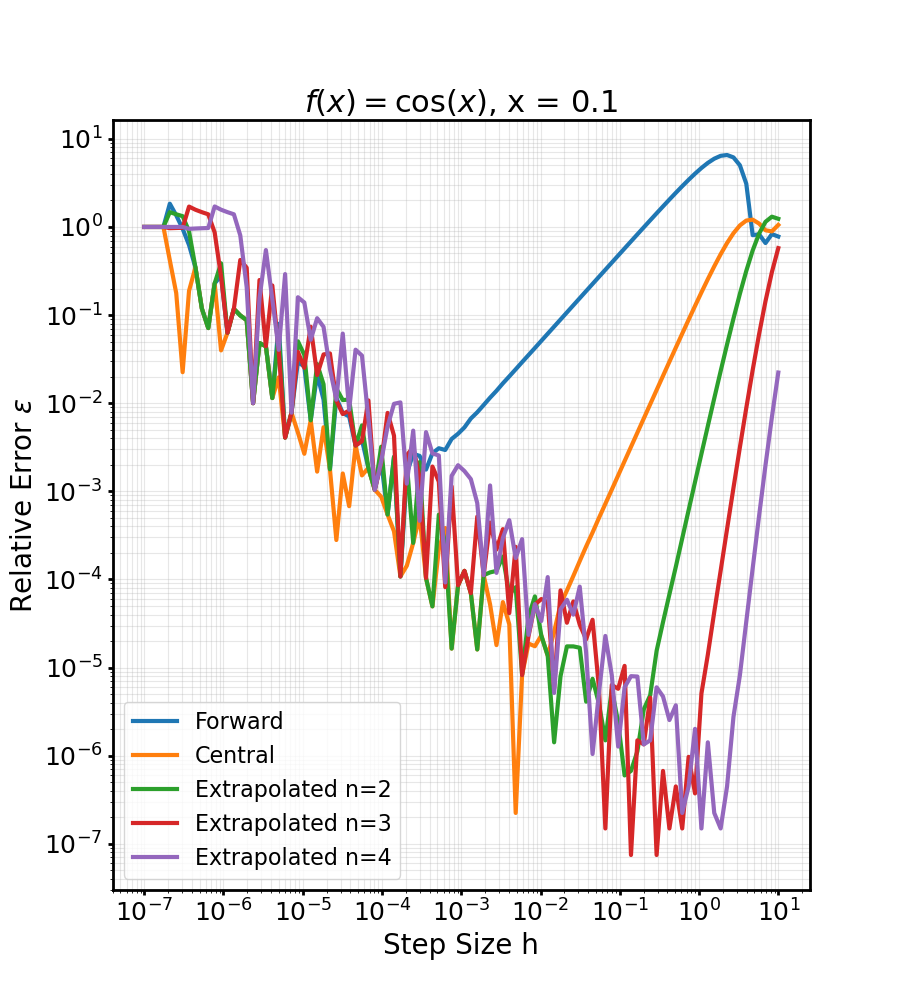
\includegraphics[width=0.48\textwidth]{figures/differentiation_results_0.1_f.png}
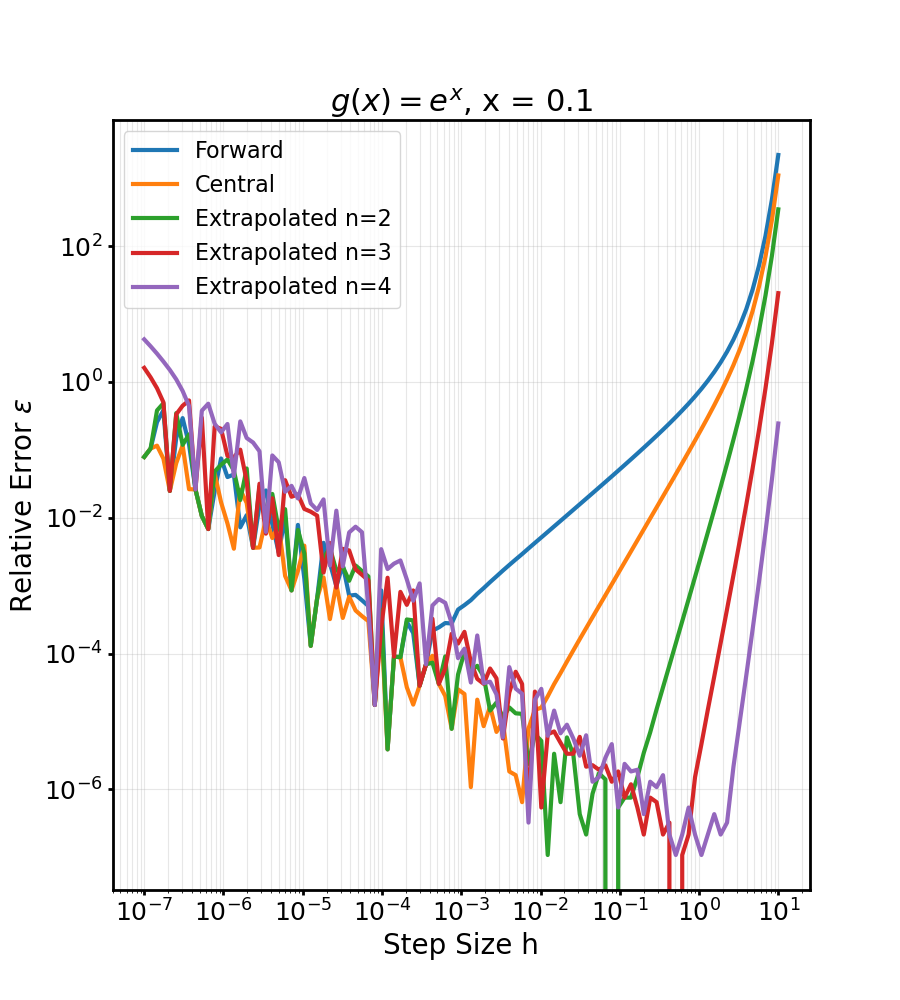
\includegraphics[width=0.48\textwidth]{figures/differentiation_results_0.1_g.png}
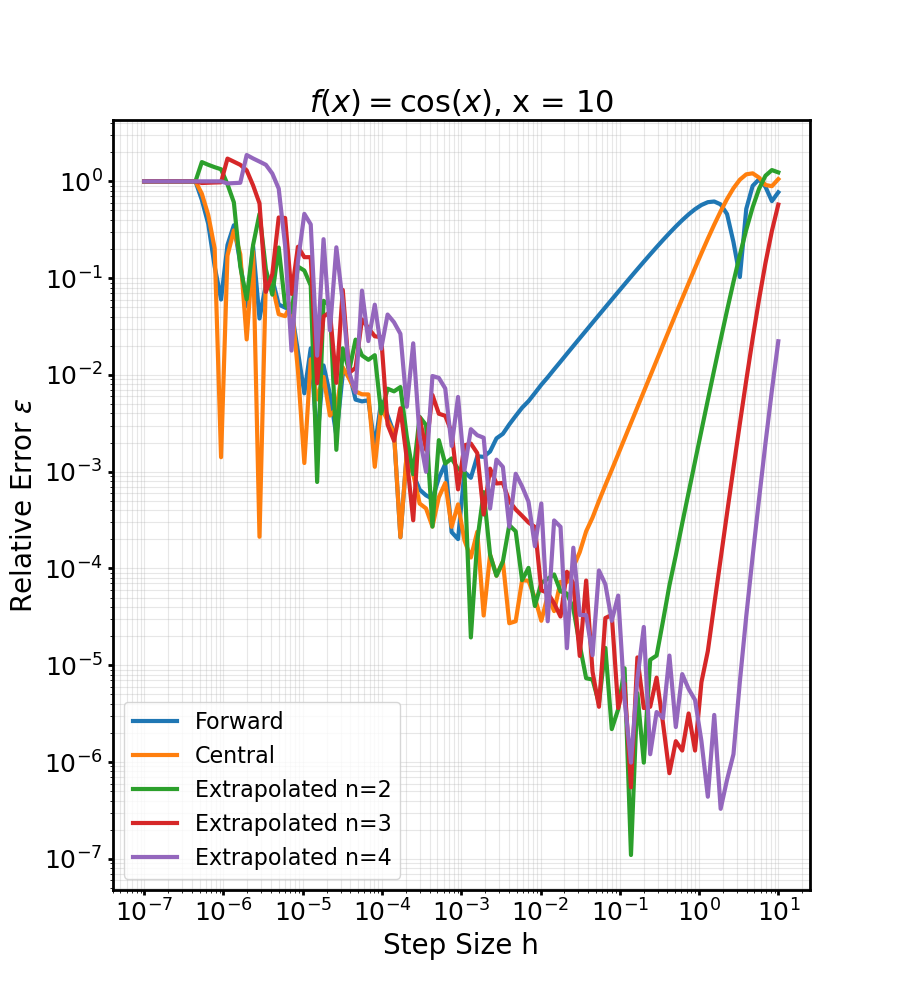
\includegraphics[width=0.48\textwidth]{figures/differentiation_results_10_f.png}
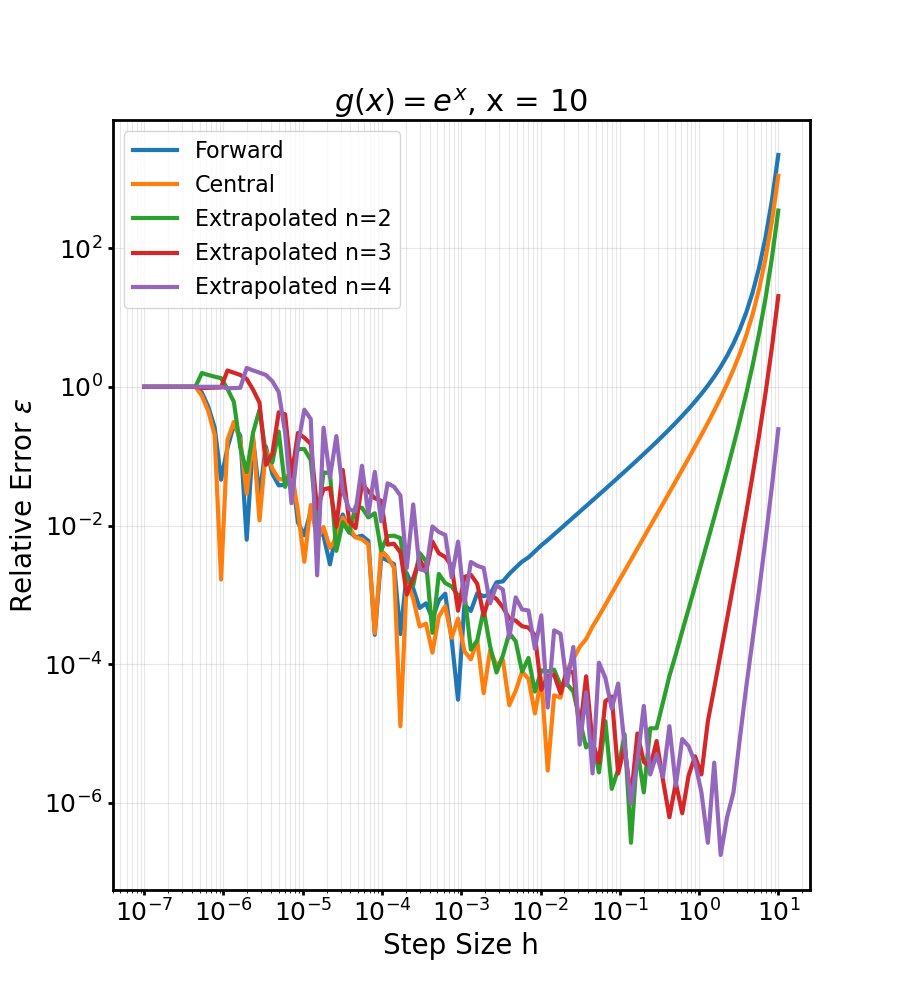
\includegraphics[width=0.48\textwidth]{figures/differentiation_results_10_g.png}
\caption{Relative error $\epsilon$ as a function of step size $h$ for the forward-, central-, and extrapolated-difference methods for $f(x)=\cos(x)$ and $g(x)=e^x$ at $x=0.1$ and $x=10$.}
\end{figure}

The number of significant digits obtained at the minimum error was estimated as $N_{\mathrm{digits}}\approx -\log_{10}(\epsilon_{\mathrm{min}}).$ For $f(x)=\cos(x)$ at $x=0.1$, the forward and central methods achieve approximately $3.97$ and $6.65$ significant digits, respectively, while the extrapolated methods with $n=2$, $3$, and $4$ achieve approximately $6.22$, $7.13$, and $6.83$ digits. For $g(x)=e^x$ at $x=0.1$, the forward and central methods achieve approximately $5.41$ and $6.19$ digits, while the $n=4$ extrapolated method reaches approximately $6.97$ digits. The $n=2$ and $n=3$ extrapolated methods produce zero measured relative error at their optimal step sizes because the numerical and analytic values become identical at single-precision, rather than implying more than the roughly seven significant digits available in single-precision.

At $x=10$, the forward and central methods give approximately $3.70$ and $4.57$ significant digits for $\cos(x)$, compared with $6.96$, $6.26$, and $6.48$ digits for extrapolation with $n=2$, $3$, and $4$. For $e^x$, the corresponding values are approximately $4.51$ and $5.53$ digits for the forward and central methods and $6.58$, $6.21$, and $6.75$ digits for the extrapolated methods. This agrees well with the expectation that higher-order methods can approach the approximately seven-digit precision limit of single-precision.

The roundoff error regime corresponds to small $h$ where the curves are spiky and irregular, meanwhile truncation error is at the latter end of the plot with the straight curves. The minimum error occurs at the transition between these two regimes. 

\subsubsection*{Round Off Error}

At small enough $h$, subtracting nearly equal floating point values causes cancelation and roundoff error to dominate. We can see this in Figure 2. The fitted slopes are close to $\epsilon \propto h^{-1}$ for all three differentiation methods and for both functions and evaluation points. The measured slopes are generally between approximately $-0.9$ and $-1.1$, in agreement with the expected $\mathcal{O}(h^{-1})$ scaling of roundoff error in a finite difference derivative.

\begin{figure}[htbp]
\centering
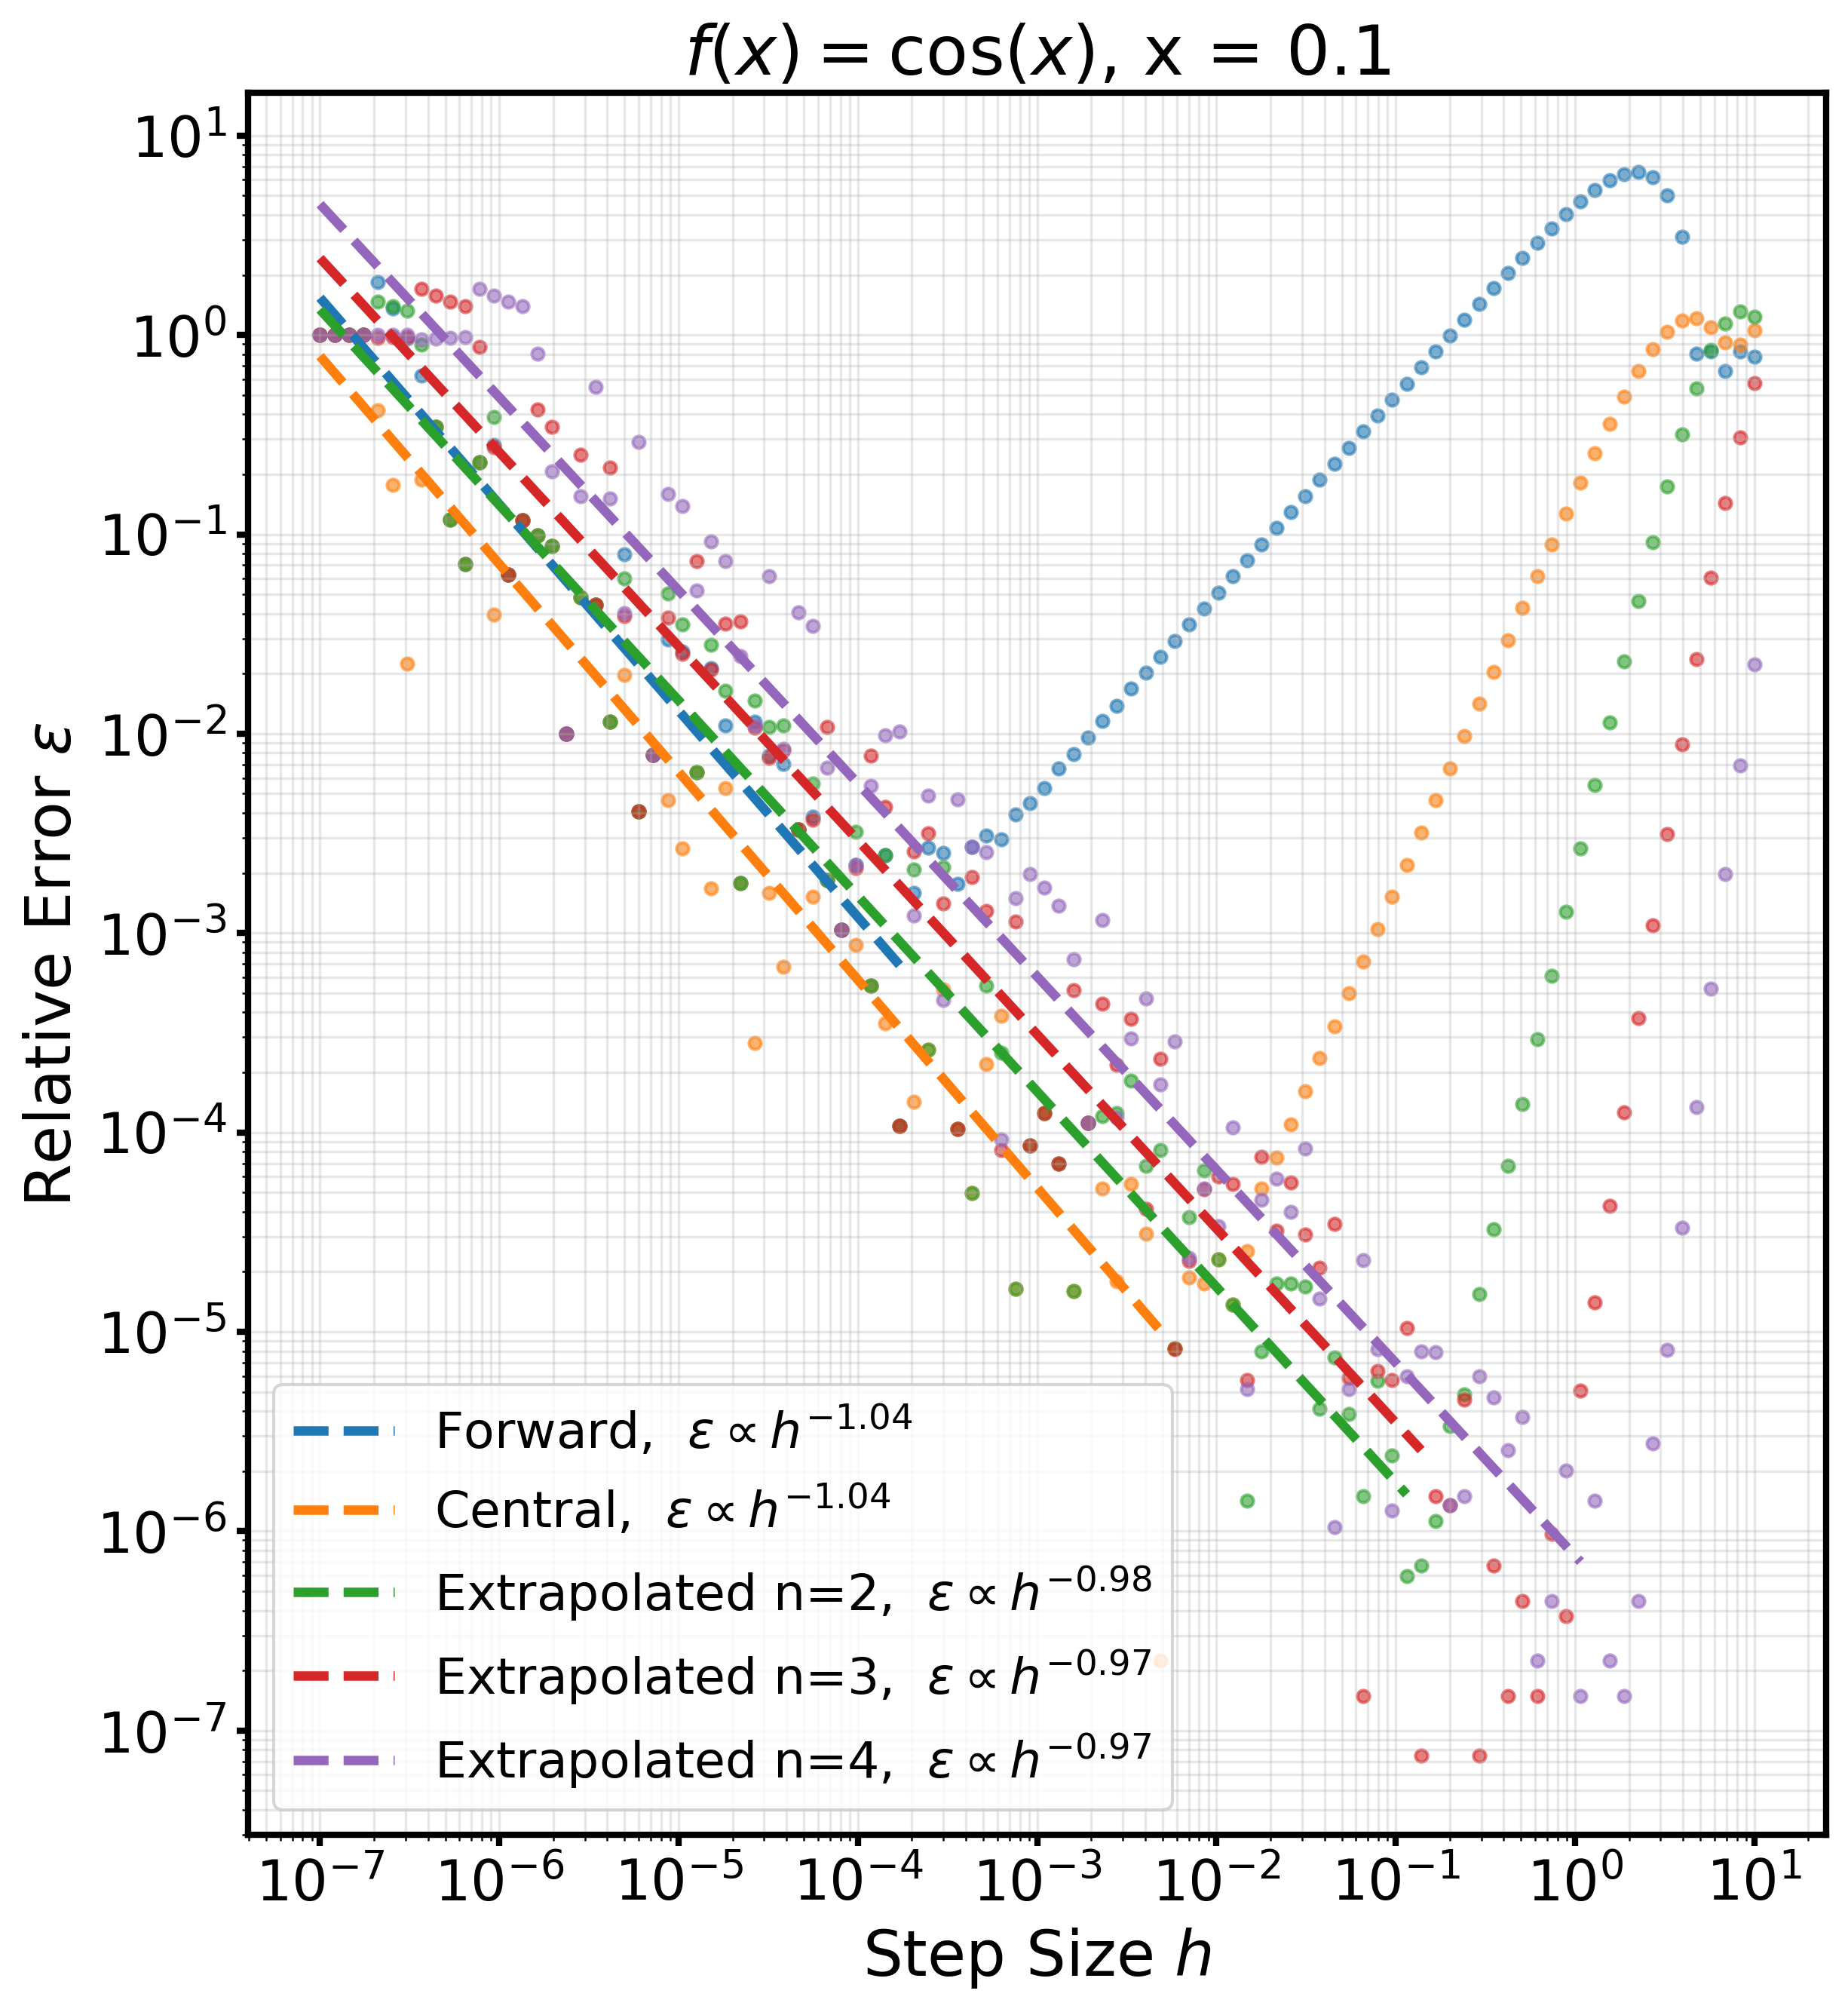
\includegraphics[width=0.48\textwidth]{figures/differentiation_roundoff_scaling_0.1_f.png}
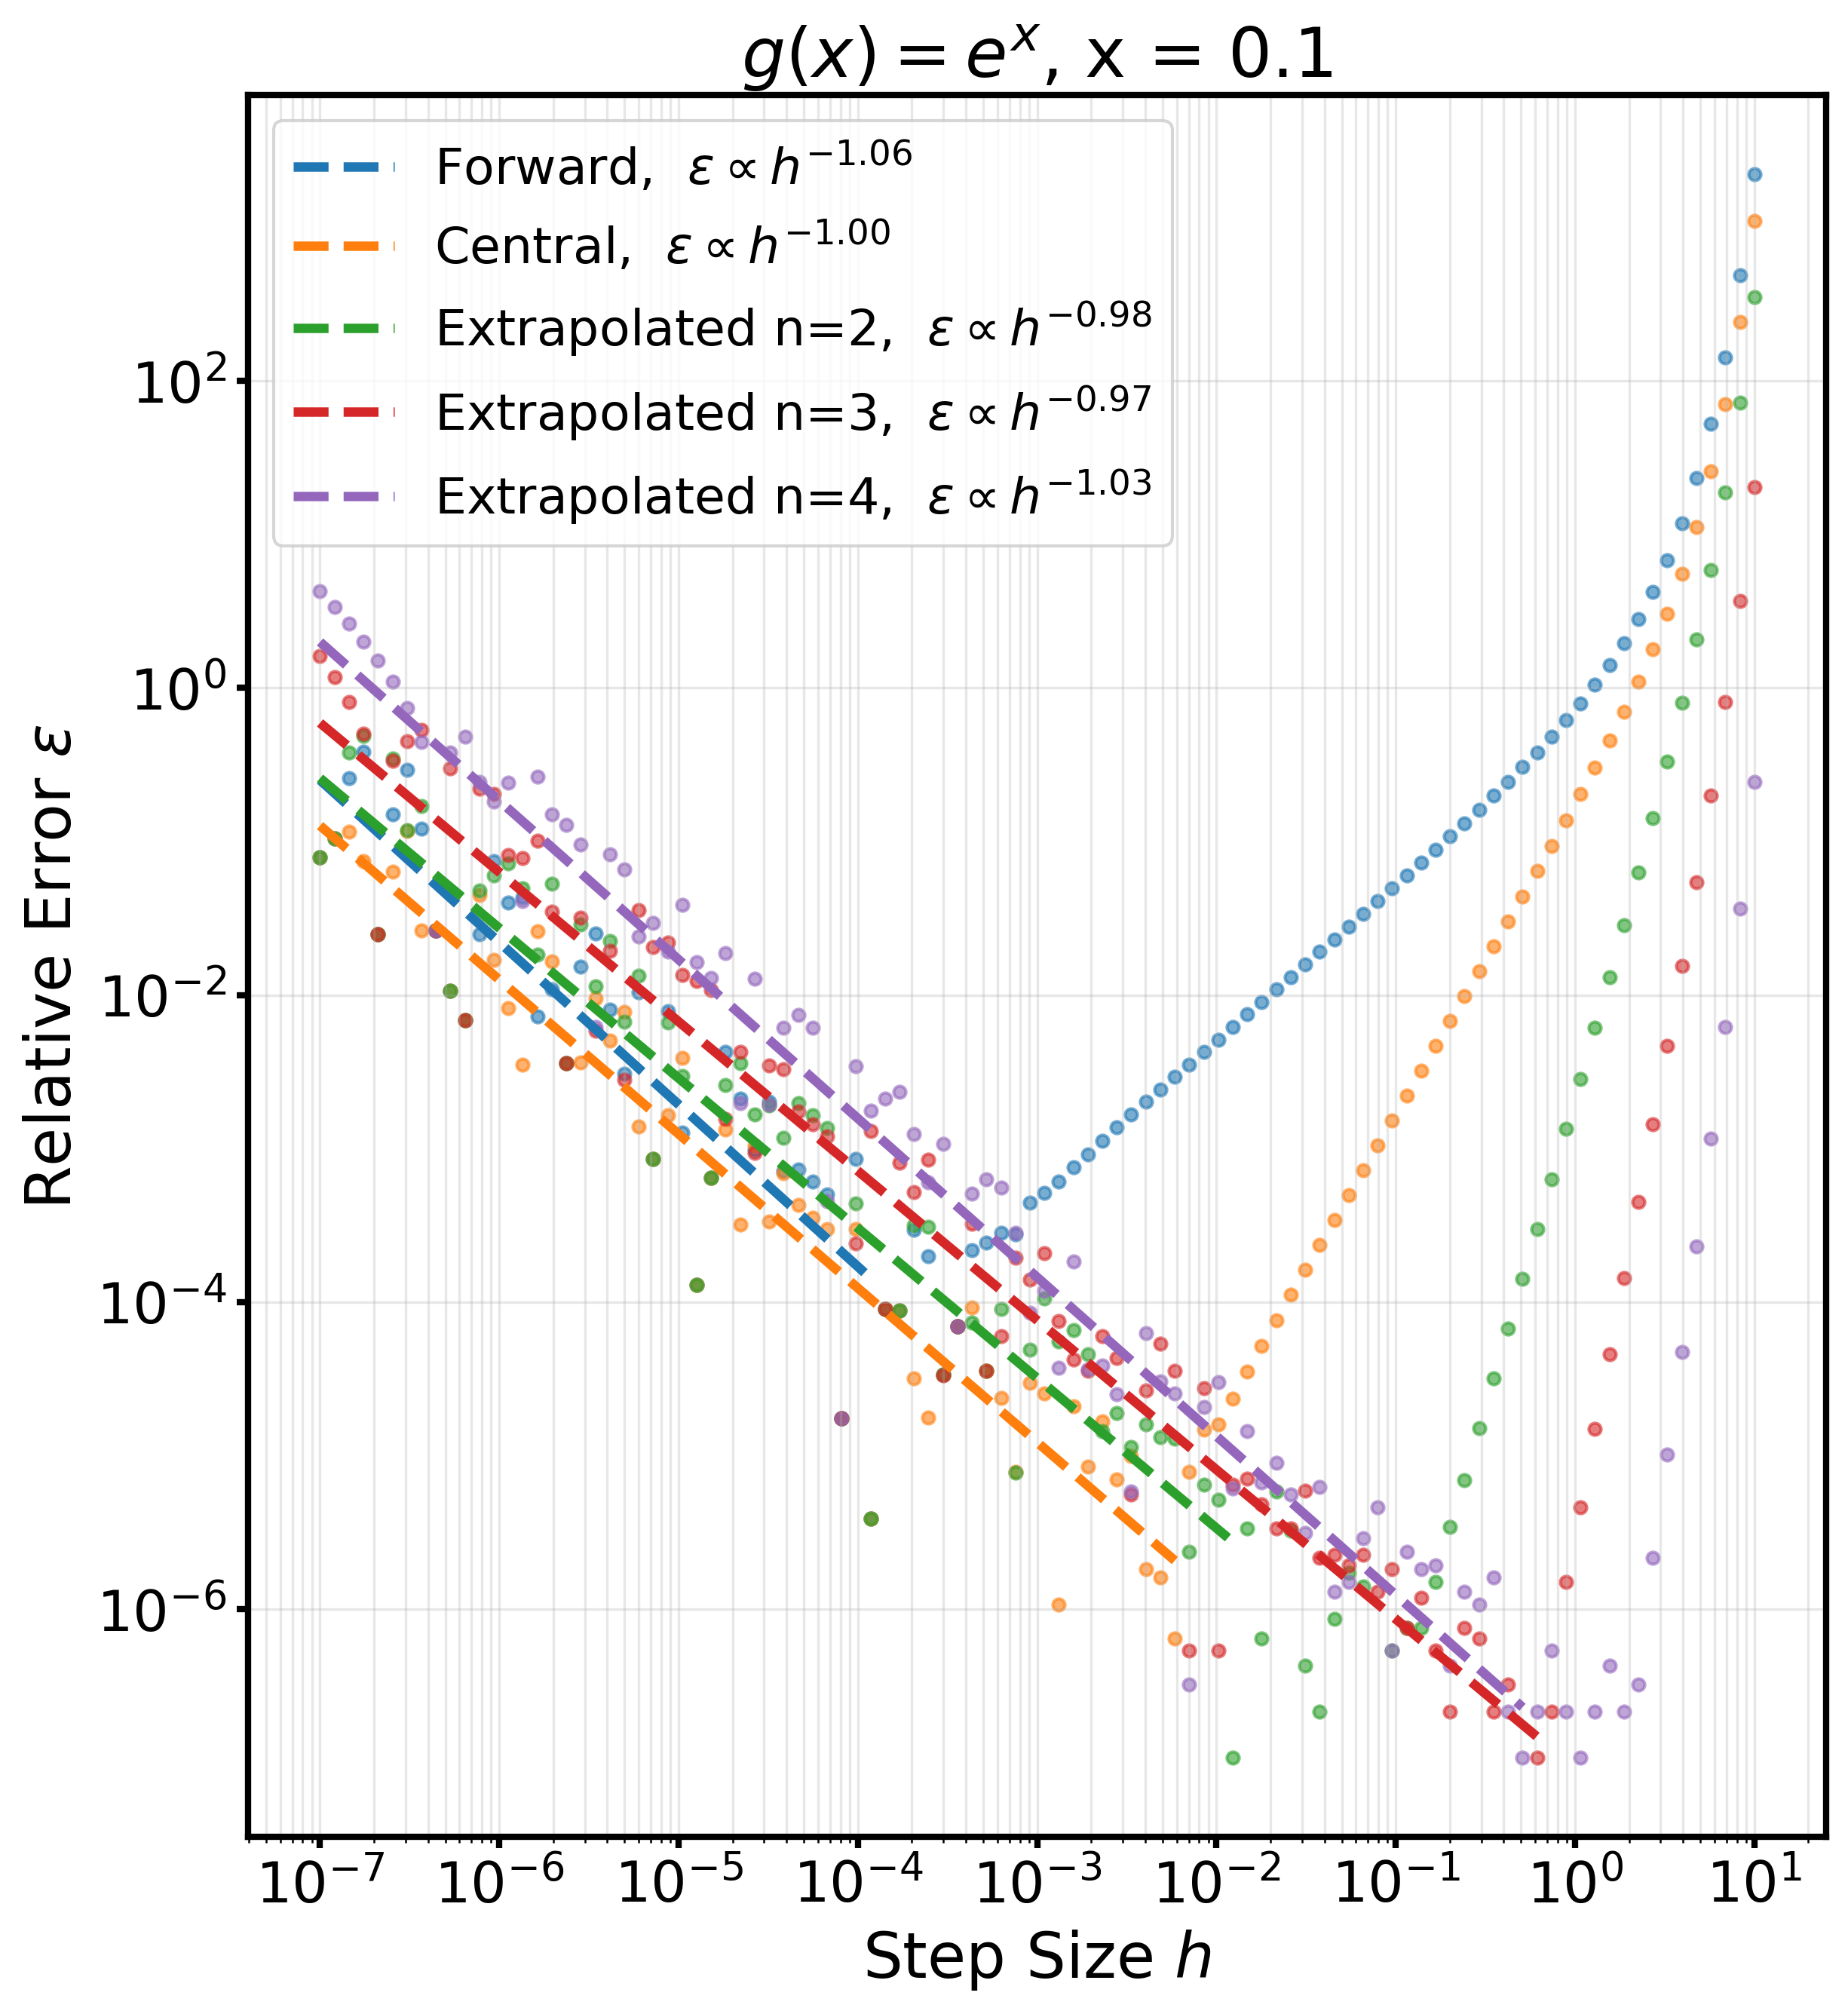
\includegraphics[width=0.48\textwidth]{figures/differentiation_roundoff_scaling_0.1_g.png}
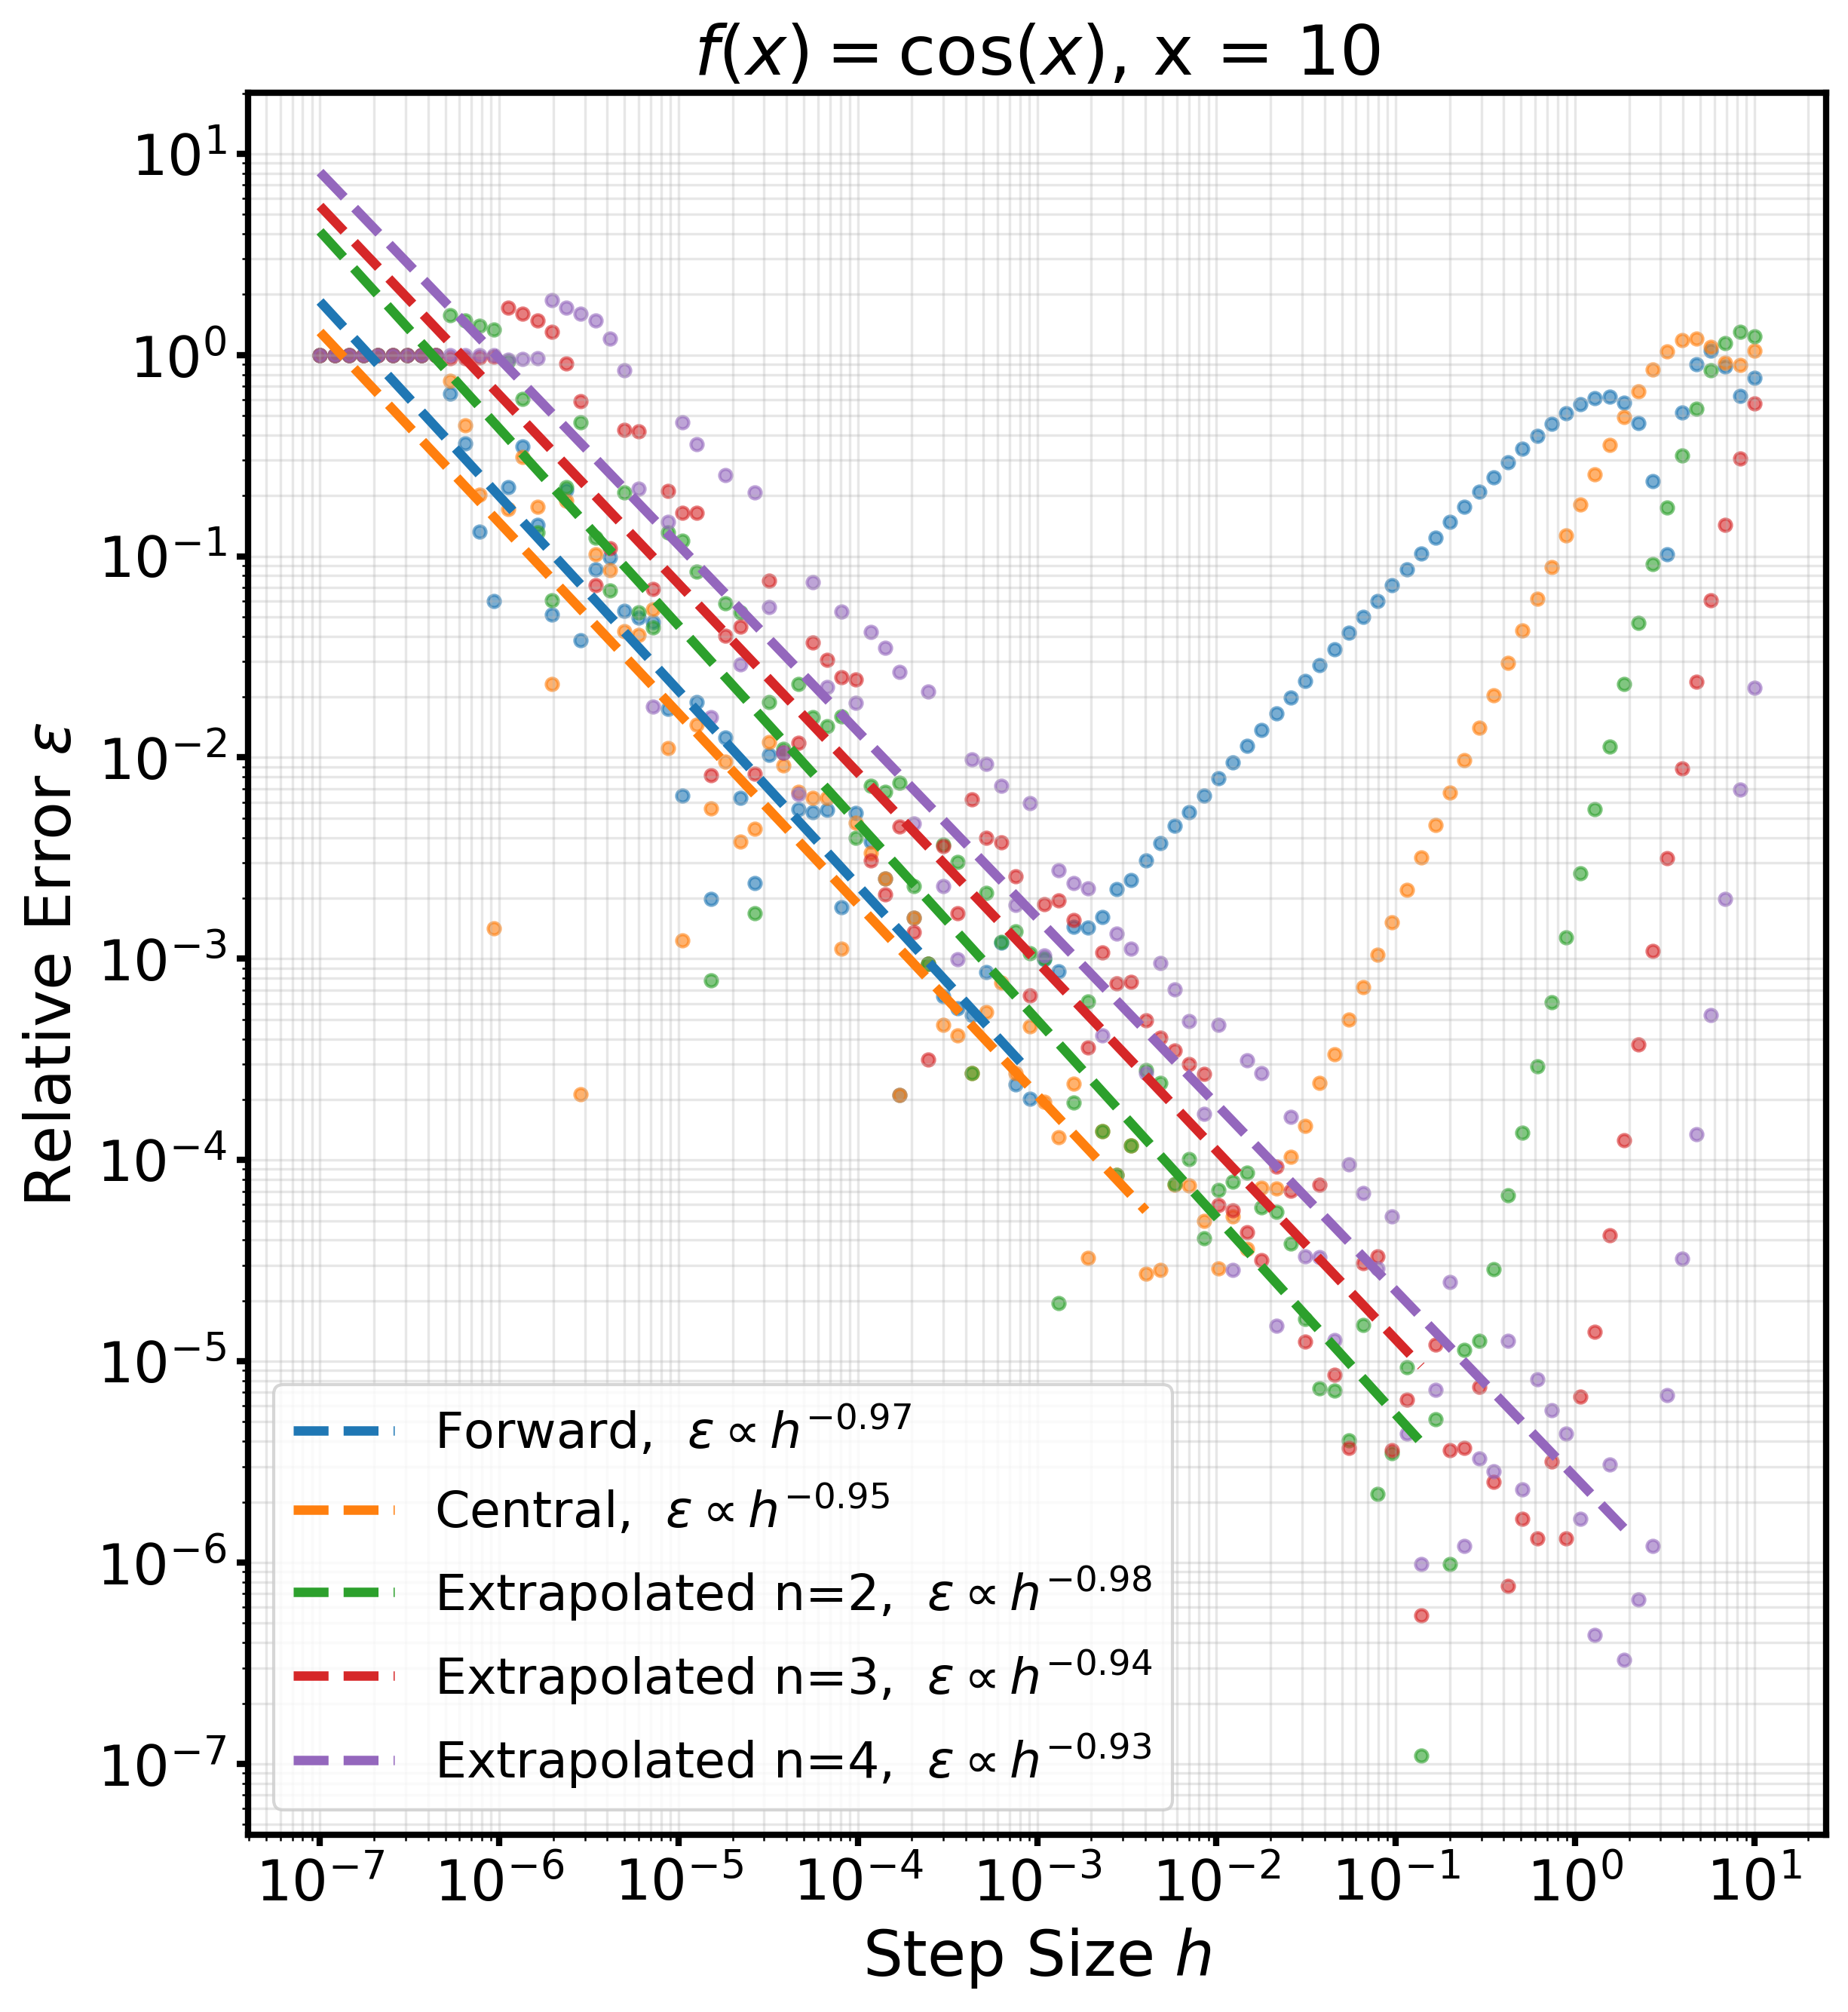
\includegraphics[width=0.48\textwidth]{figures/differentiation_roundoff_scaling_10_f.png}
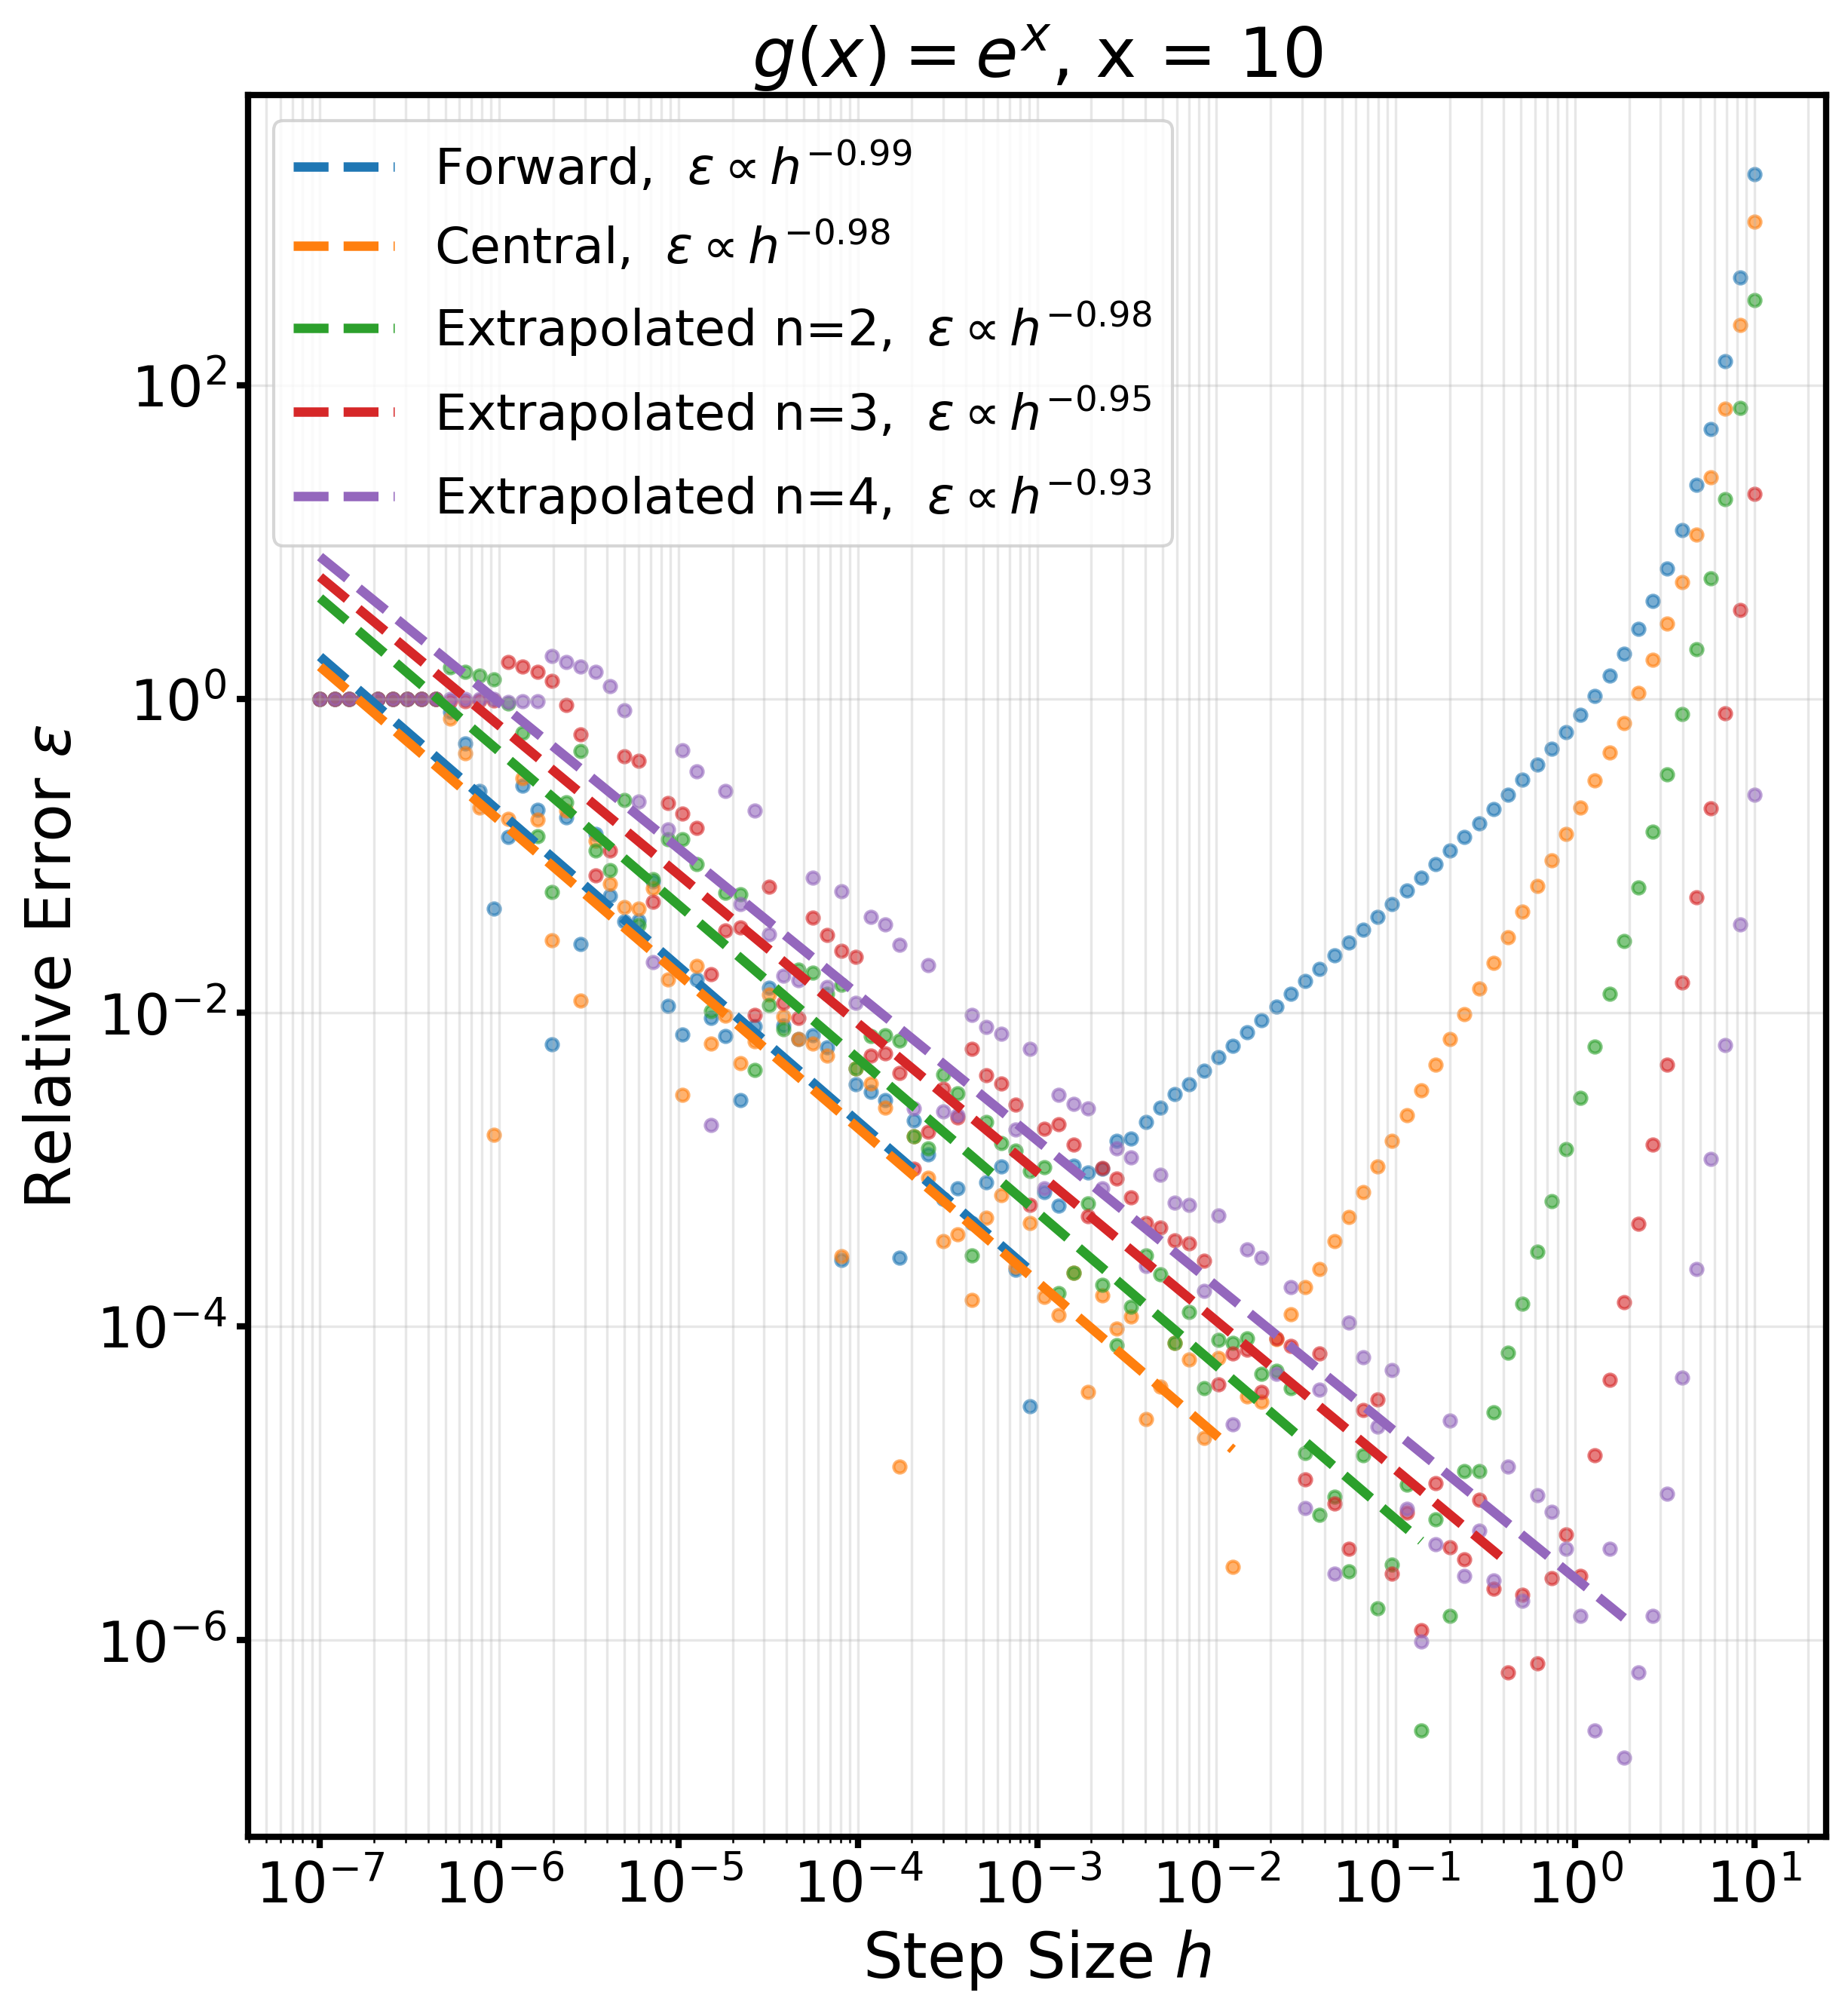
\includegraphics[width=0.48\textwidth]{figures/differentiation_roundoff_scaling_10_g.png}
\caption{Relative error in the small-$h$ roundoff-dominated regime. The fitted slopes are close to $\epsilon\propto h^{-1}$ for the forward-, central-, and extrapolated-difference methods.}
\end{figure}

\subsubsection*{Truncation Error}

At larger $h$, truncation error overpowers roundoff error and the measured error scalings follow the expected order of each method. Figure 3 shows that the forward-difference error scales approximately as $\epsilon \propto h,$ while the central-difference error scales approximately as $\epsilon \propto h^2.$

The extrapolated methods give progressively steeper scalings of about $\epsilon_{n=2}\propto h^4$, $\epsilon_{n=3}\propto h^6$, and $\epsilon_{n=4}\propto h^8$.

The fitted exponents vary slightly between the two functions and evaluation points, but are close to the expected orders.

\begin{figure}[htbp]
\centering
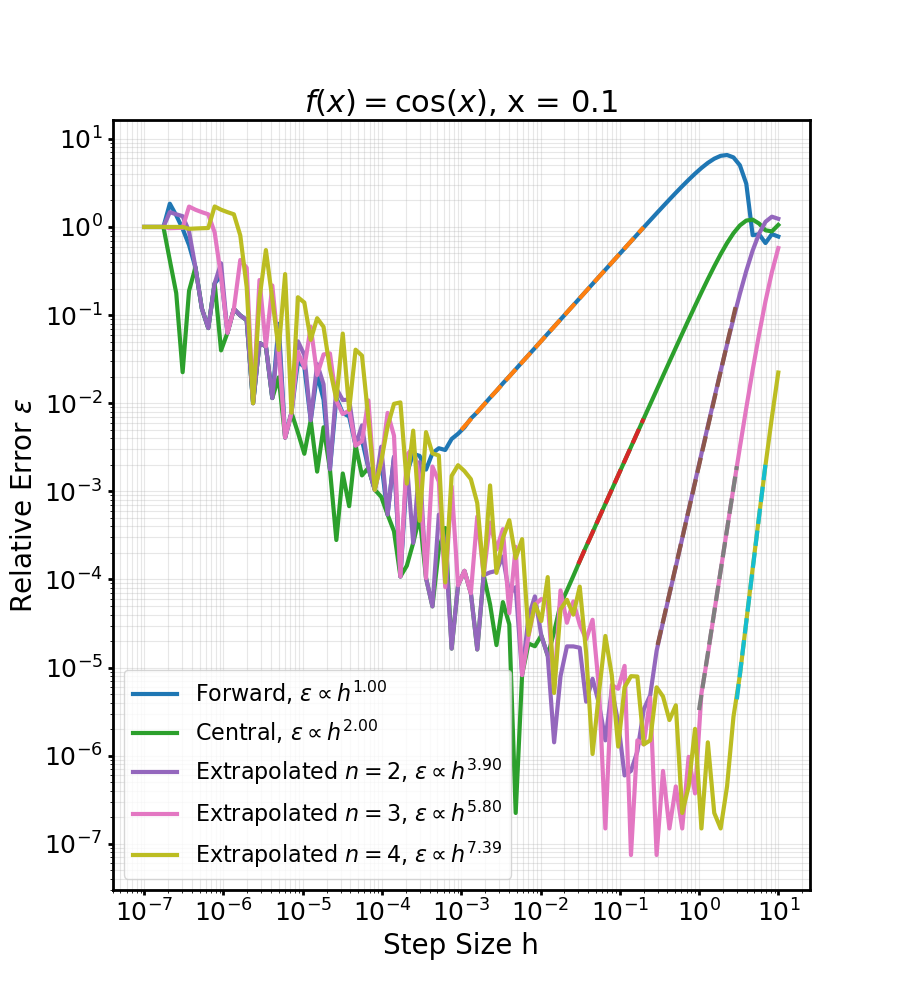
\includegraphics[width=0.48\textwidth]{figures/differentiation_scaling_0.1_f.png}
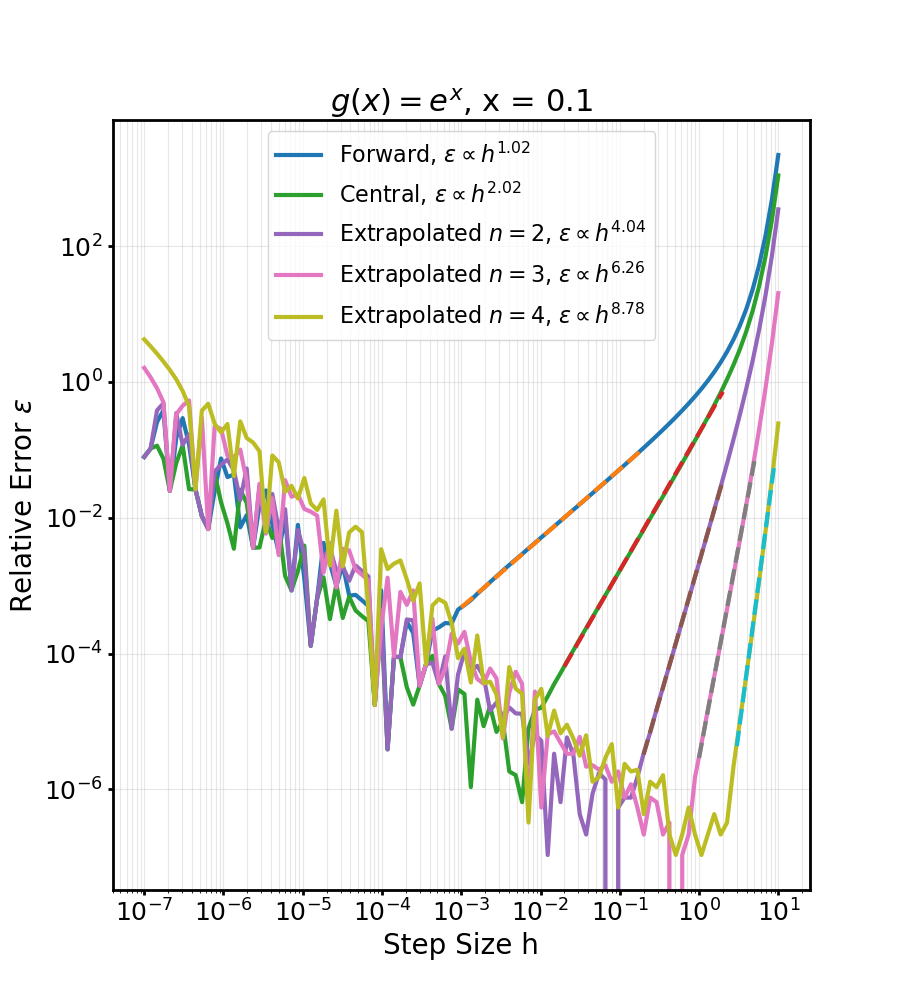
\includegraphics[width=0.48\textwidth]{figures/differentiation_scaling_0.1_g.png}
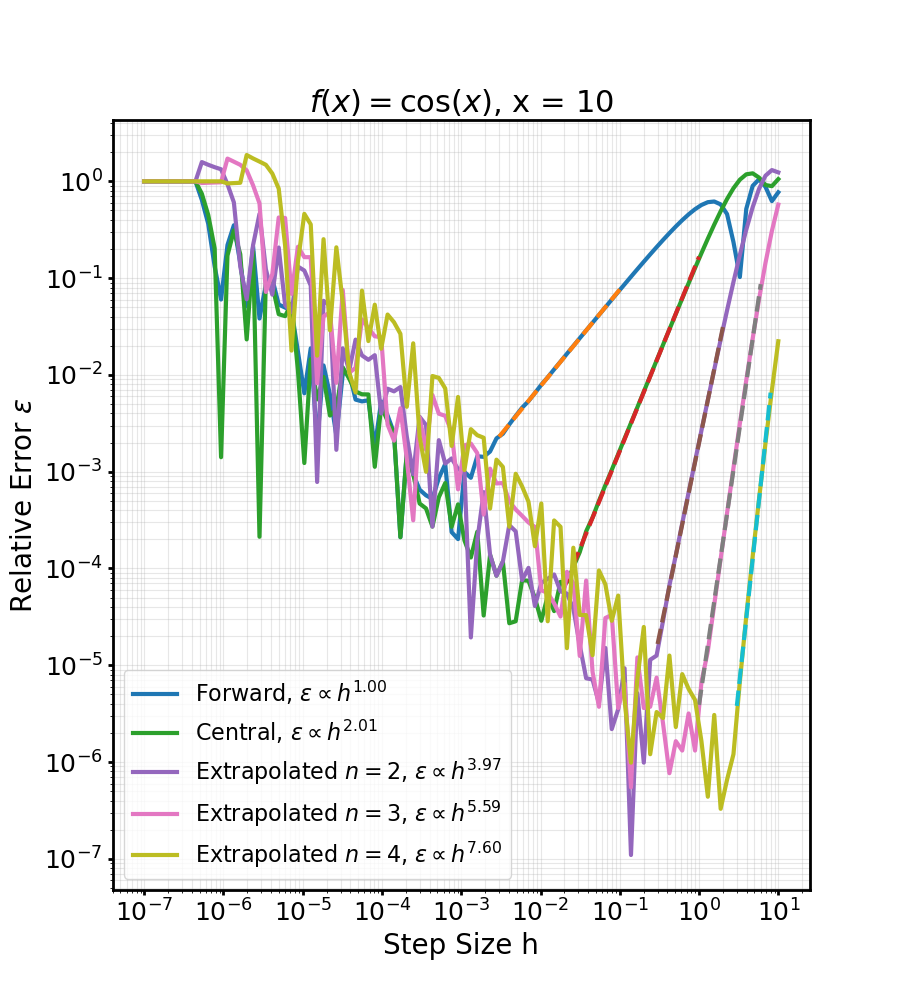
\includegraphics[width=0.48\textwidth]{figures/differentiation_scaling_10_f.png}
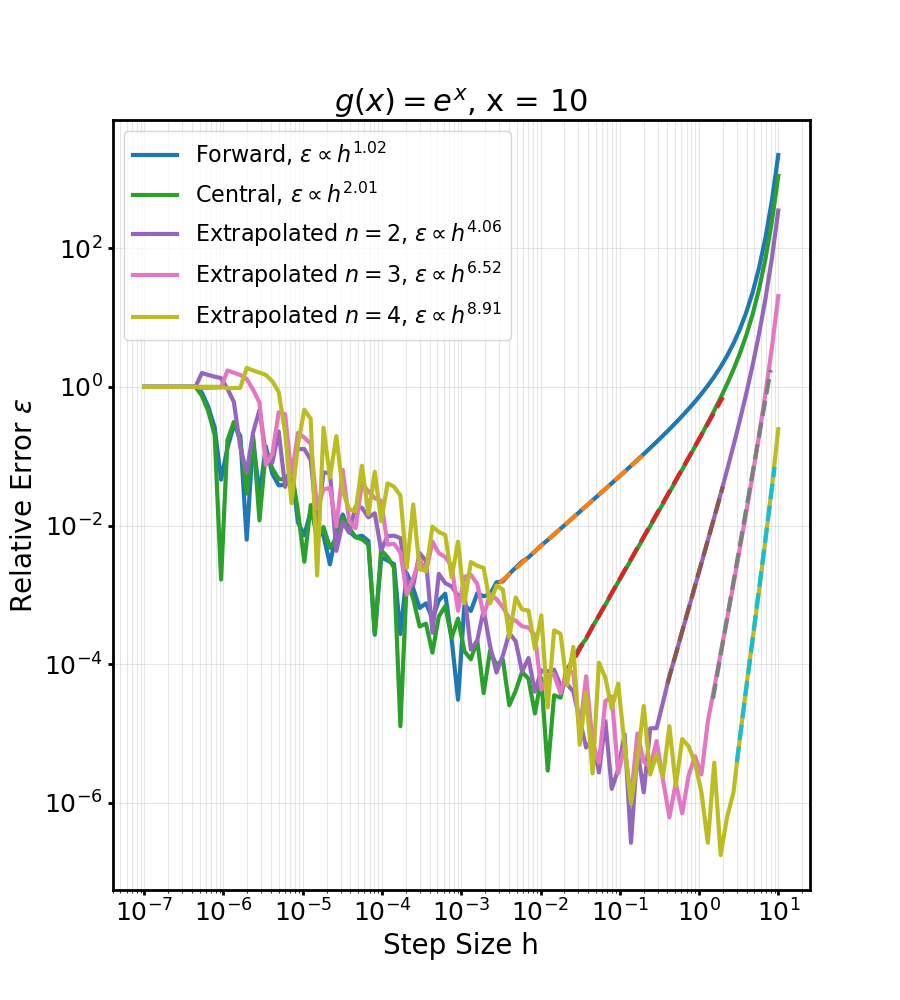
\includegraphics[width=0.48\textwidth]{figures/differentiation_scaling_10_g.png}
\caption{Relative error in the truncation error dominated regime. The forward and central methods scale approximately as $h$ and $h^2$, while successive Richardson extrapolations approach $h^4$, $h^6$, and $h^8$.}
\end{figure}

\subsection*{Numerical Integration}

Figure 4 shows the relative error as a function of the number of integration bins $N$ for the midpoint, trapezoidal, and Simpson's rules. At small and intermediate $N$, the midpoint and trapezoidal errors decrease approximately as $\epsilon \propto N^{-1.99},$
which matches the expected $\mathcal{O}(N^{-2})$ truncation error. Simpson's rule decreases more rapidly as $\epsilon \propto N^{-3.96},$ which is close to the expected $\mathcal{O}(N^{-4})$ scaling.

At large enough $N$, increasing the number of bins no longer improves the result because the truncation error becomes smaller than the roundoff error. The curves therefore flatten and become irregular rather than continuing along their original slopes. Simpson's rule reaches this roundoff-dominated regime with fewer bins because its truncation error decreases more rapidly.

\begin{figure}[htbp]
\centering
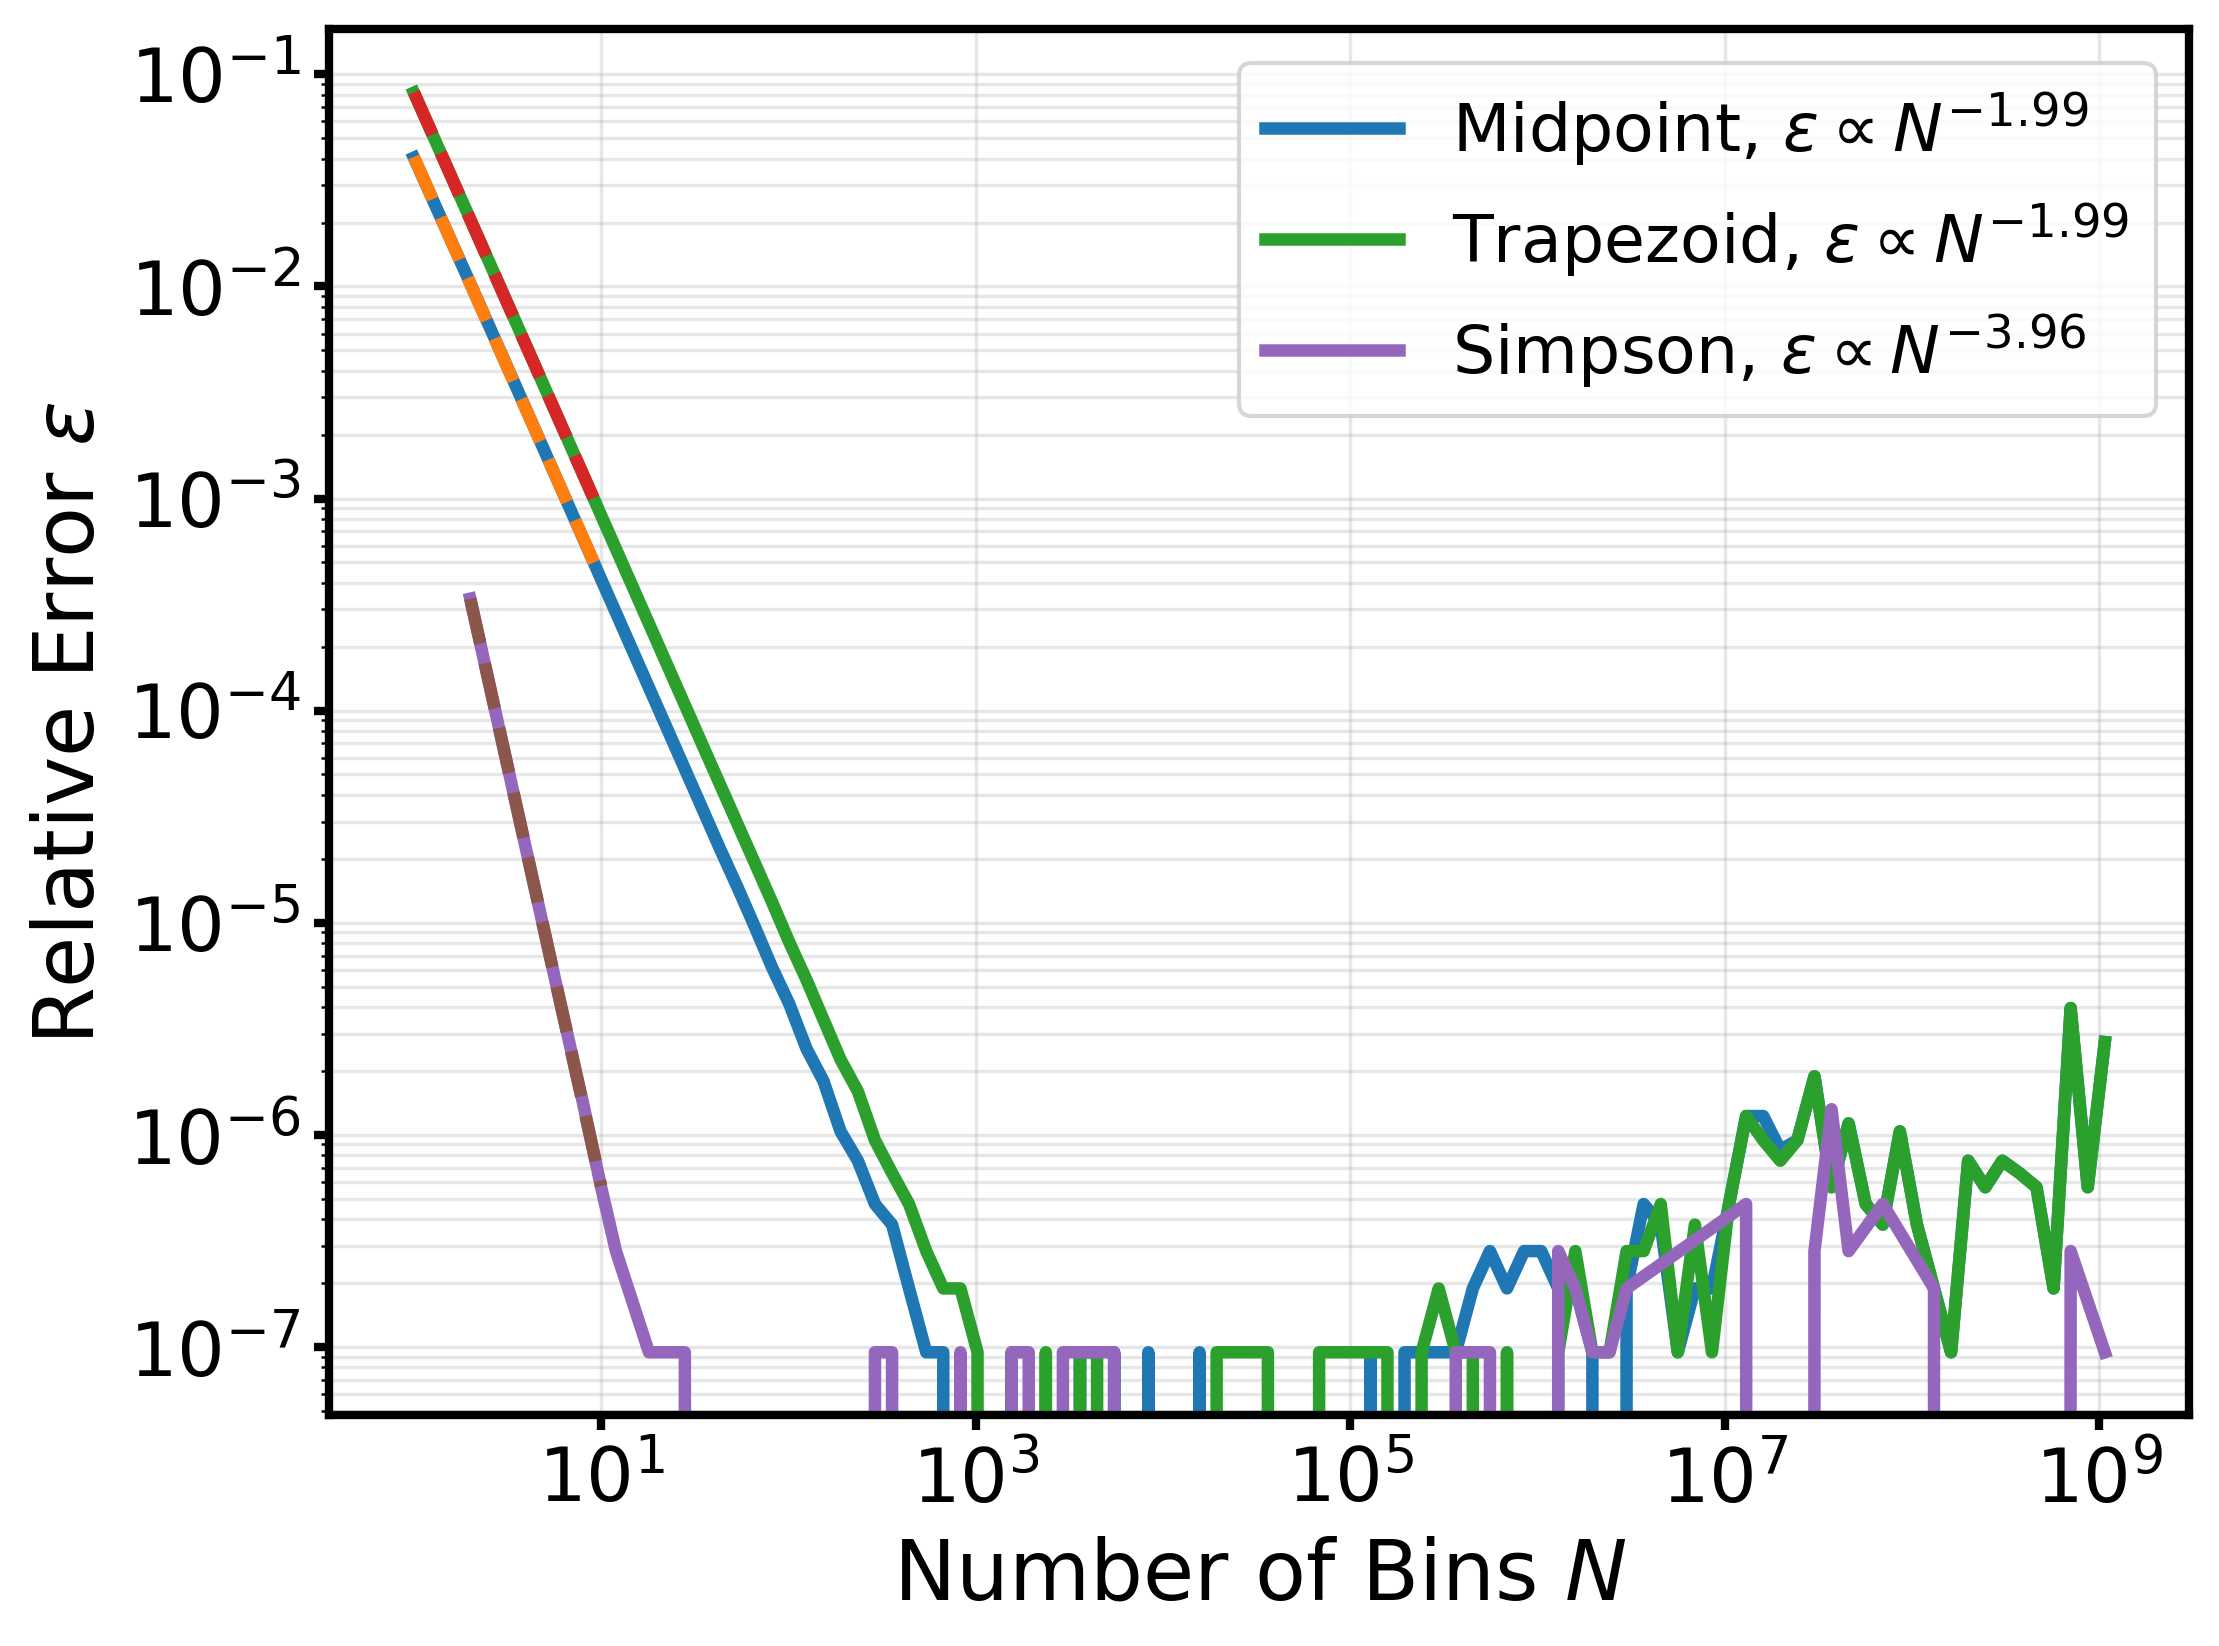
\includegraphics[width=0.75\textwidth]{figures/integration_results.png}
\caption{Relative integration error $\epsilon$ as a function of the number of bins $N$ for the midpoint, trapezoidal, and Simpson's rules. The fitted truncation-error scalings are approximately $N^{-2}$ for the midpoint and trapezoidal rules and $N^{-4}$ for Simpson's rule. At large $N$, roundoff error limits further improvement.}
\end{figure}

\subsection*{Baryon Acoustic Oscillations}

Figure 5 shows the matter power spectrum and its linear and cubic-spline interpolations. The two interpolation methods follow the same overall shape of $P(k)$, although there is a bit of an offset in the value of $P(k)$ at small $k$.

\begin{figure}[htbp]
\centering
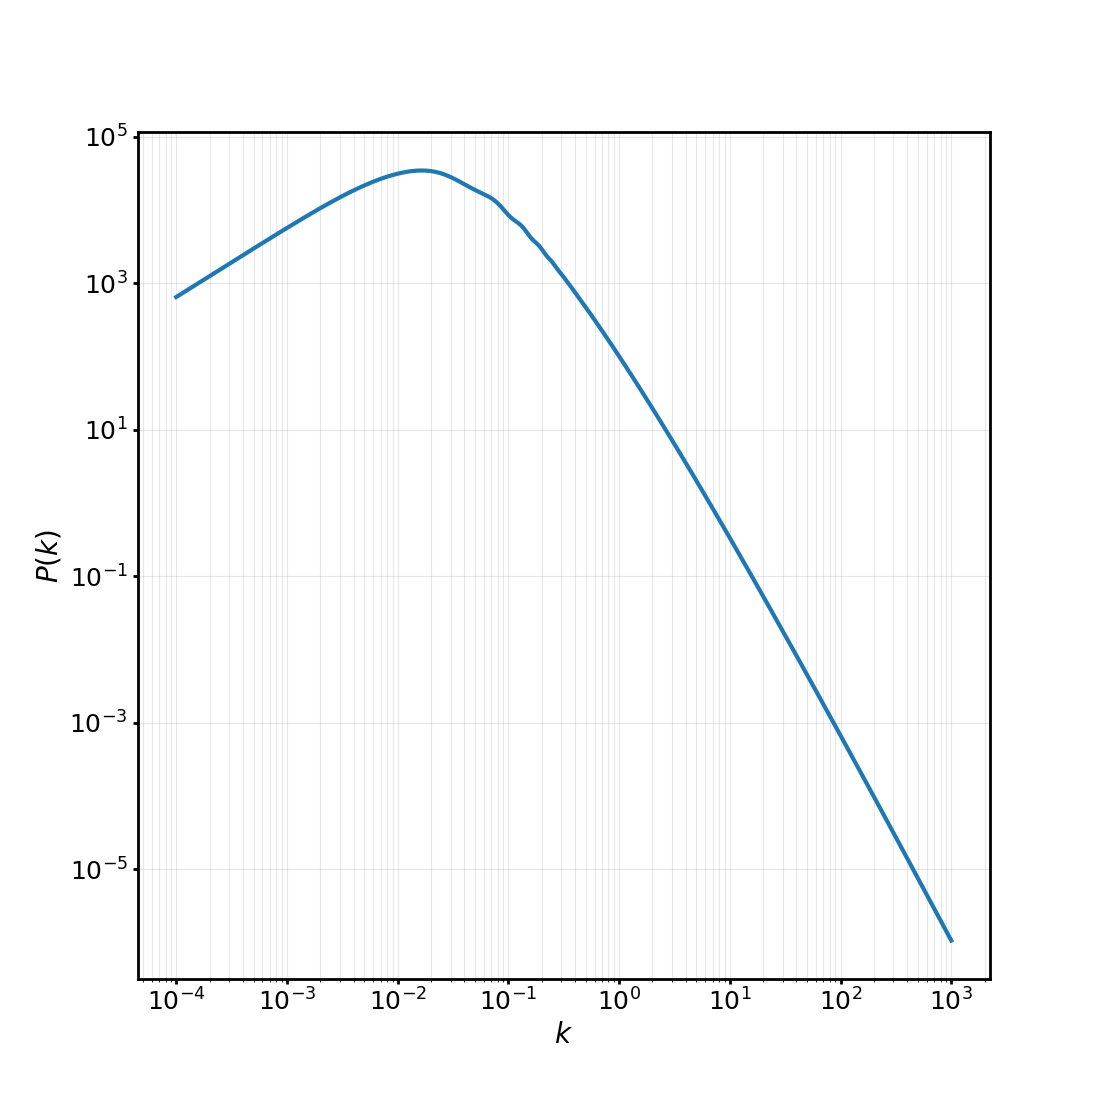
\includegraphics[width=0.48\textwidth]{figures/power_spectrum.png}
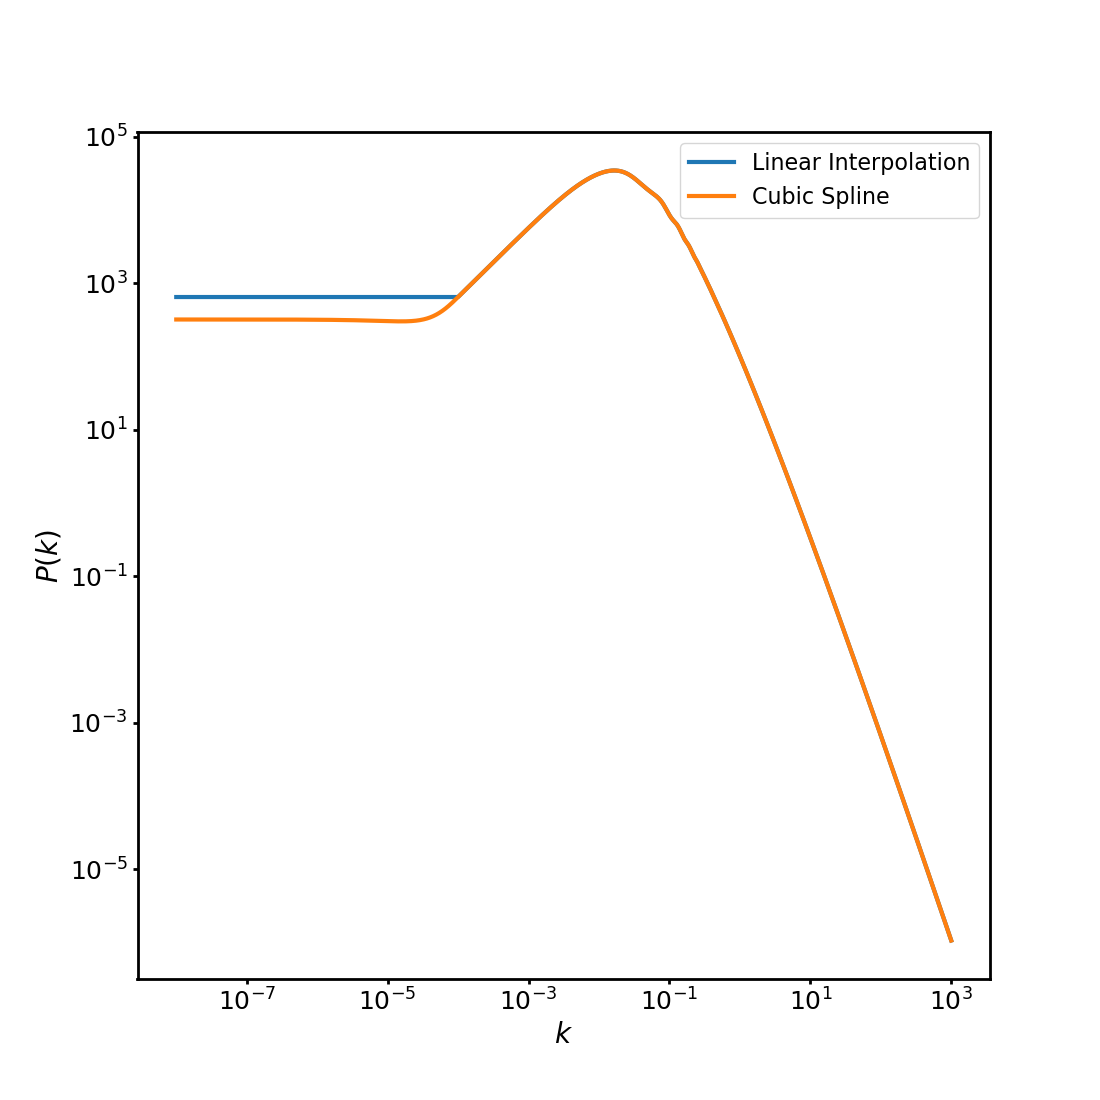
\includegraphics[width=0.48\textwidth]{figures/interpolation.png}
\caption{Matter power spectrum $P(k)$ and comparison between the linear and cubic-spline interpolation methods.}
\end{figure}

Figure 6 shows $r^2\xi(r)$ obtained from the cubic-spline and linear interpolations, together with the fractional difference between the resulting correlation functions. Both interpolation methods extract the BAO peak at
\[ r_{\mathrm{BAO}} \approx 105.64\ \mathrm{Mpc}/h. \] The cubic-spline interpolation gives a peak value of $r^2\xi(r)\approx18.03$, while the linear interpolation gives approximately $17.92$. Thus, although the interpolation method produces small differences in the value of the correlation function, the inferred BAO scale is unchanged.

\begin{figure}[htbp]
\centering
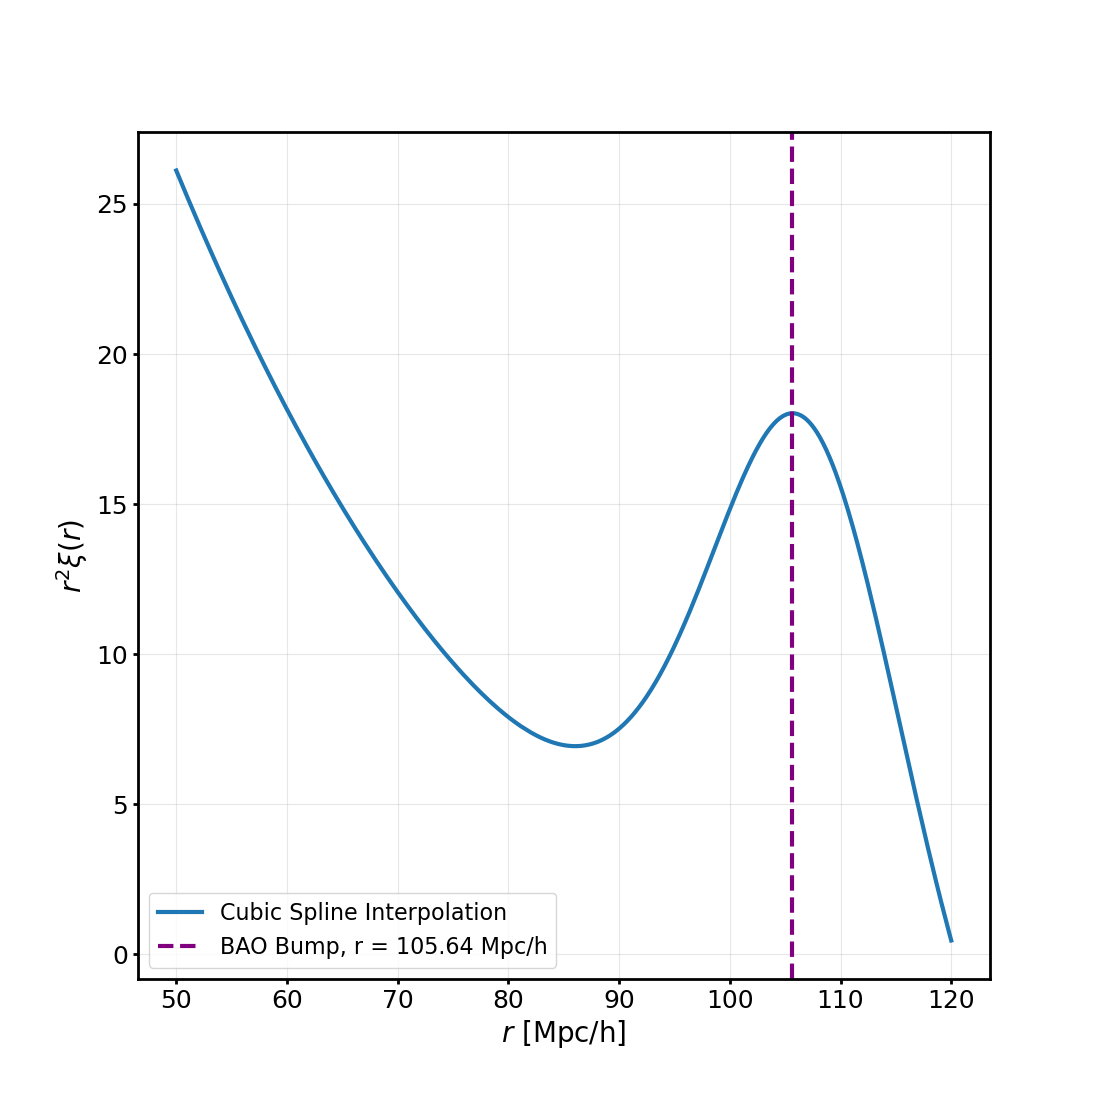
\includegraphics[width=0.48\textwidth]{figures/correlation_function_cubic.png}
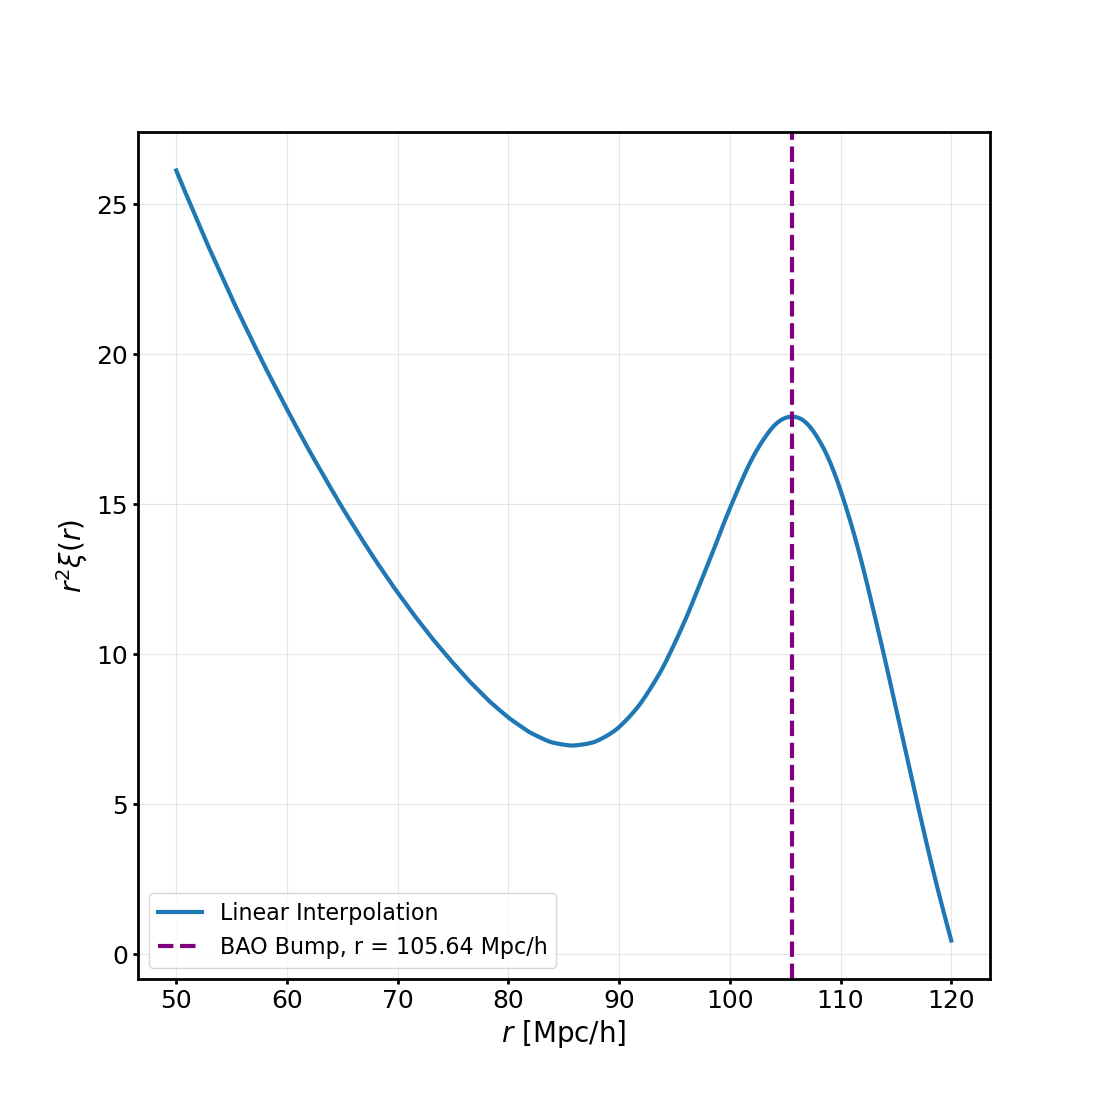
\includegraphics[width=0.48\textwidth]{figures/correlation_function_linear.png}
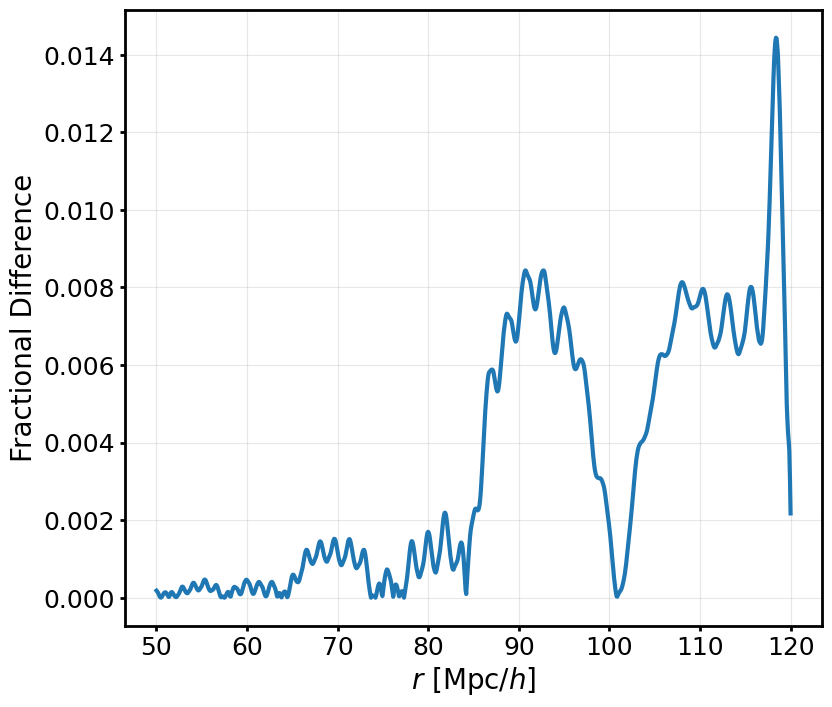
\includegraphics[width=0.8\textwidth]{figures/correlation_function_fractional_error.png}
\caption{Correlation function obtained using cubic-spline and linear interpolation of the matter power spectrum, together with their fractional difference. Both methods locate the BAO peak at approximately $105.64$ Mpc$/h$, while giving slightly different values of $\xi(r)$.}
\end{figure}

\section*{Code}

The link to the github repository for this homework assignment can be accessed by clicking \href{https://github.com/jpalmagomez/computational_physics_homework_1.git}{here}.

\clearpage

\end{document}